\documentclass[]{article}

\usepackage[margin=1.2in]{geometry} 
\usepackage{url} 
\usepackage{parskip}
\usepackage{graphicx}
\usepackage{float}

\begin{document}

\title{Queensland Crime Data Analysis}
\author{Roy Portas - s4356084}
\date{\today}
\maketitle 
\section{Introduction}

Criminology is the study of causes, nature and prevention of criminal behaviour\cite{roufa_early_nodate}.
This study is important as it allows sociologists and psychologists to not only study the when and how crime occurs, but offers a way to predict crime trends in the future.

Crime is an evident part of our society and is an active topic during elections\cite{remeikis_queensland_2016}, even companies like IBM\cite{noauthor_ibm_2012} and Palantir\cite{palantir_technologies_law_nodate} 
are creating products to model, predict and prevent crimes before they happen.

As technology becomes more powerful and less expensive, the cost of implementing systems capable of predicting crimes becomes more feasible.
However building these systems are difficult due to the sheer amount of data that needs processing.
Nevertheless companies have started building such systems.

Crime prediction systems generally consist of the following components:
\begin{itemize}
    \item Identify areas with frequent crime\cite{noauthor_ibm_2012}
    \item Match trends in national and regional crimes with local crimes
    \item Identify circumstances for the cause of crimes\cite{noauthor_ibm_2012}
\end{itemize}

\section{Aims}

This report aims to analyse and explore crime data for Queensland. A variety of techniques and datasets will be used to explore this problem, including:

\begin{itemize}
    \item Analyse monthly offences to determine correlations during certain months of the year.
    \item Analyse reported offences by suburb, month and offence type to find relationships in crime over time.
    \item Analysis of geolocation data for crime locations and police districts to find divisions with high crime.
\end{itemize}

\section{Methods}

\subsection{Data Sourcing}

The data was downloaded from the Queensland Government data website, \url{data.qld.gov.au}. 
The following table shows the data sources used for this report.

\begin{table}
    \centering
    \begin{tabular}{|p{4cm}|p{10cm}|}
        \hline
        Data Source & URL \\
        \hline
        QPS Police Stations & https://data.qld.gov.au/dataset/qps-police-stations \\ 
        Offence numbers by police division & https://data.qld.gov.au/dataset/offence-numbers-police-divisions-monthly-from-july-2001 \\
        \hline
    \end{tabular}
\end{table}

The files were provided as CSV and Shapefiles, which are both common storage formats for this kind of data.
The files are maintained and updated by Queensland Police, who update it every month with new crime data.
As this data comes directly from the Queensland Police service, it should be accurate and reliable.
The data is accurate to individual months and police divisions, which gives more than enough detail to model crimes in Queensland.
Both CSV and Shapefiles are easy to import into Matlab, thus are suitable datasets to use.

\subsection{Data Processing}

The first dataset used is the offence rates per police division\cite{noauthor_offence_nodate}, which is a CSV file with 65000 rows and 90 columns.
This is a lot of data to process, thus the data was preprocessed and saved in a Matlab format (.mat).
This allowed the data to be easily loaded without having to process it again.
Since the dataset has 90 dimensions, it is impossible to visualize it, so the total number of offences was found.
This simple method of dimensionality reduction allowed easy plotting of the data to find crime trends in districts over time.

The second dataset is stored in a Shapefile format, which is a common format for geospatial vector data.
This dataset was also preprocessed, as the shapefile stores the points of every boundary for every police region in Queensland.
With the data processed, a map was created showing the boundaries of every police district in Queensland, see  figure~\ref{fig:police_divisions} for a visualization of the boundaries.

Both datasets use police divisions, thus allows the datasets to be joined.
However the formatting of the police divisions are inconsistent,
with one dataset using \verb|BRISBANE CITY| with the other using \verb|Brisbane City|. 
This was fixed by converting all the names to lowercase.

\subsection{Data Analysis}

\section{Results}

\subsection{Analysing historic crime data for Queensland}

The offences per district were aggregated into totals for every month.
This shows the total number of offences in Queensland each month between January 2001 and December 2016.
Since the data consists of values over a set of months, it makes sense to visualise it as a heatmap, with months on the x axis, years on the y axis and the color of the resulting box being the intensity of crimes during that time.
This allows easy inspecting of the data to compare the amount of crime occurring during the year and how it compares to other years.

\begin{figure}[H]
    \caption{Heatmap of crime over time}
    \centering
    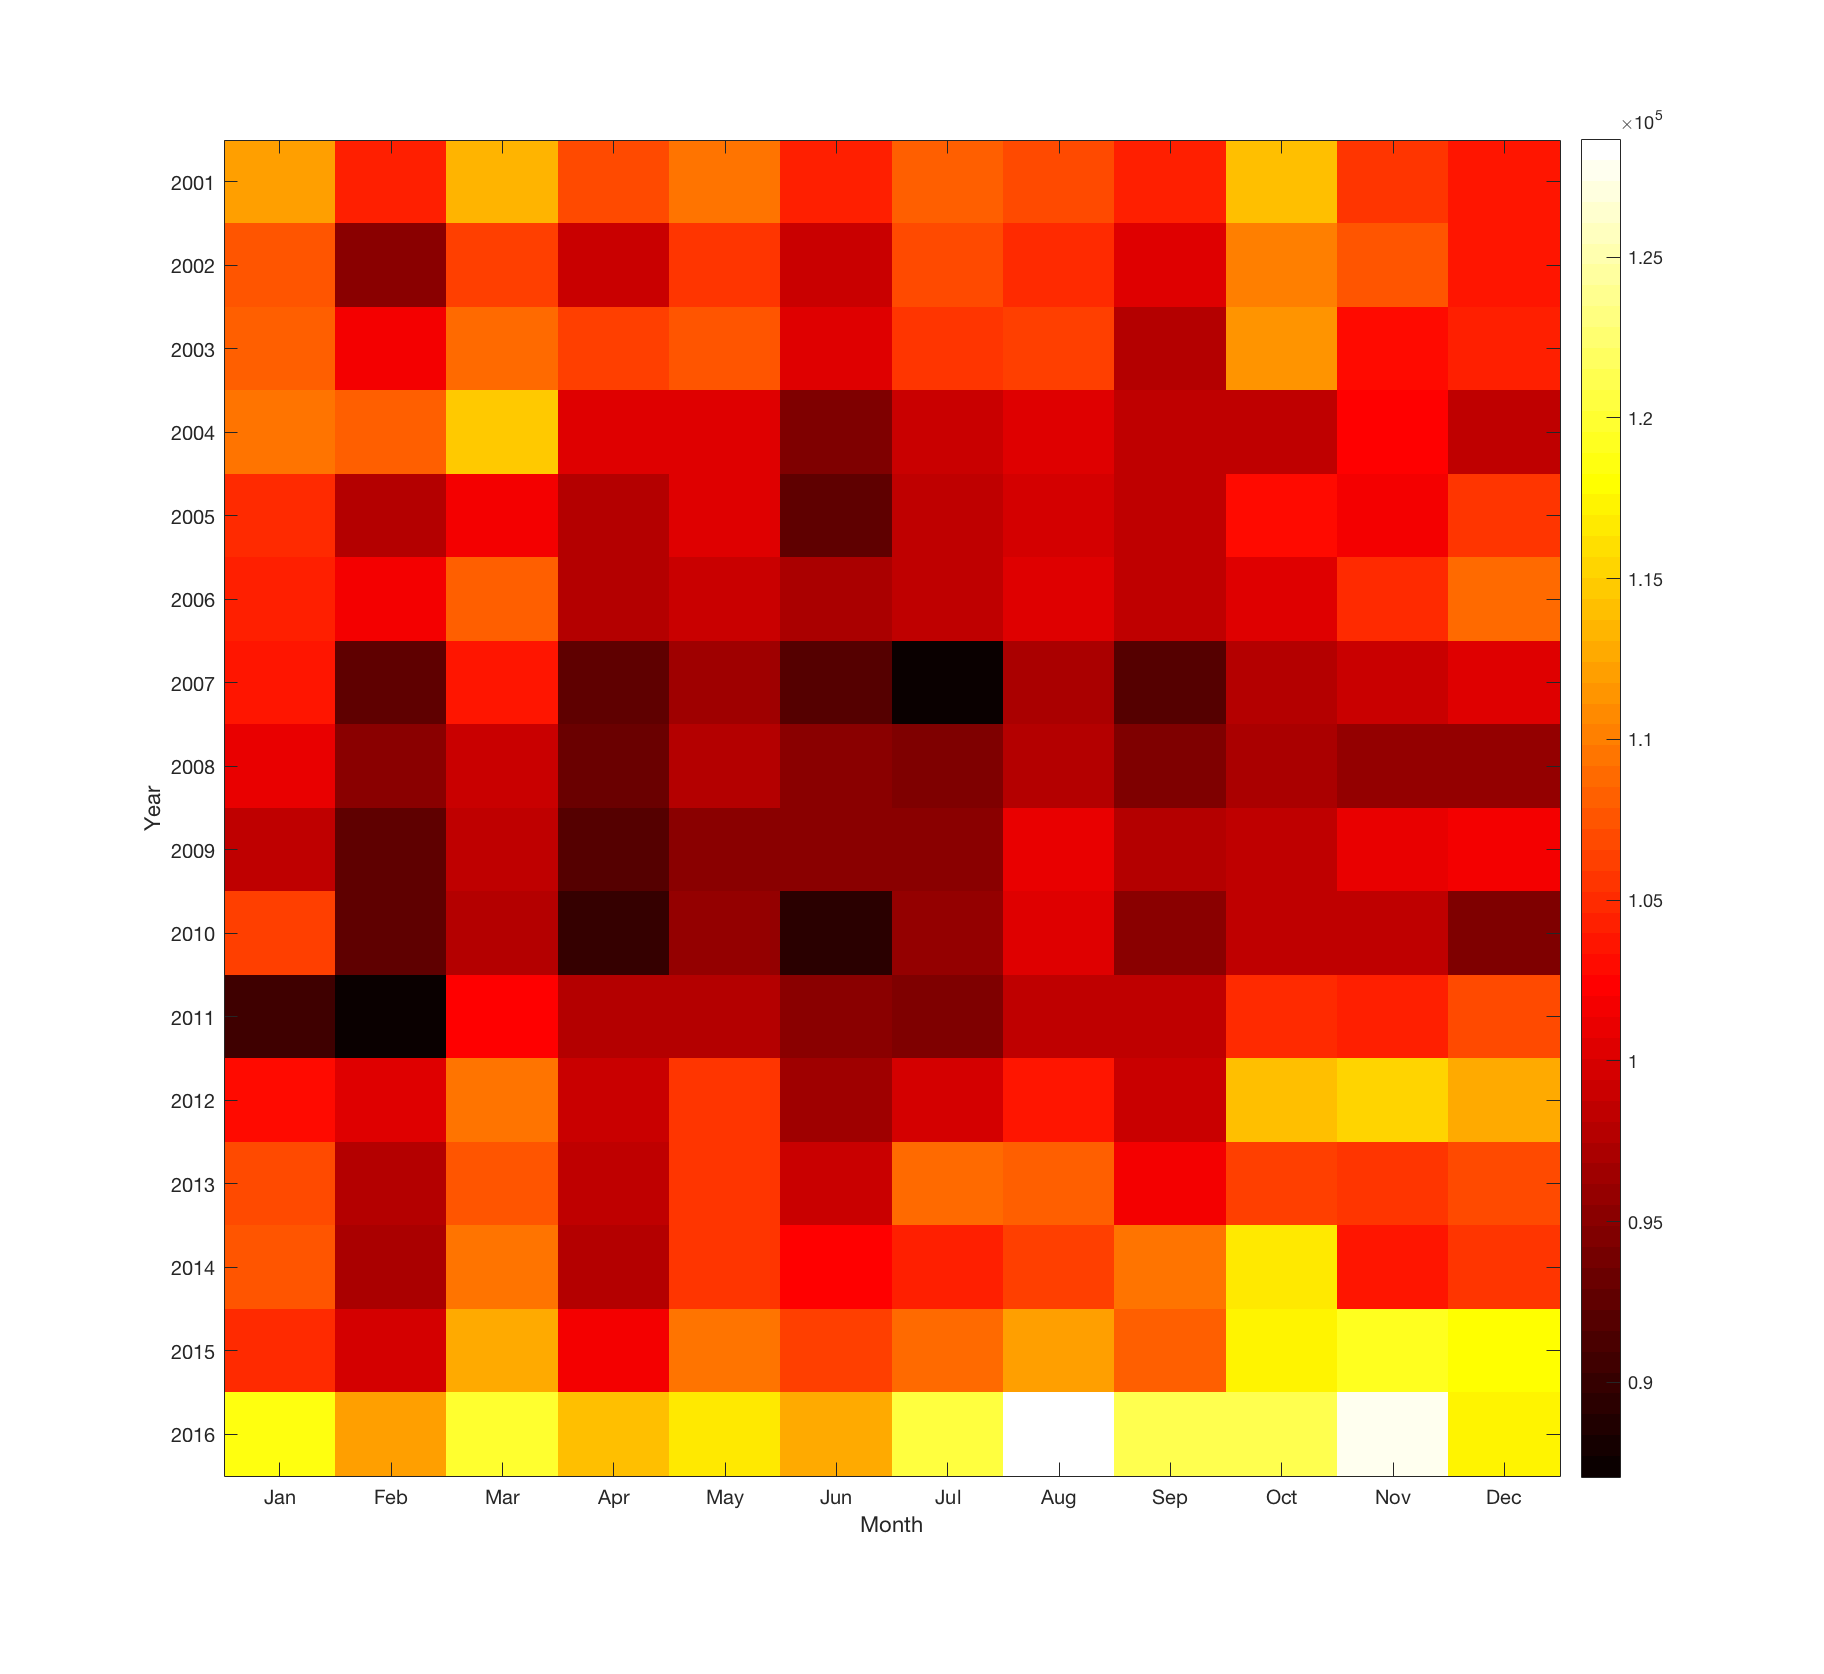
\includegraphics[width=\linewidth]{../images/crime_time_heatmap}
\end{figure}

The heatmap shows that more crime occurs during October, November, December and January than the other months. 
Additionally overall offences has been steadily increasing since 2014, with
2016 having by far the most offences for any year on record.
August and November of 2016 has spikes in the number of offences.

The data also shows a significant drop in crime from December 2010 to February 2011.
This correlates with the 2010-2011 floods in Queensland, in which three quarters of the council areas
in Queensland became disaster zones\cite{noauthor_201011_2017}.
The heatmap indicates that crime dramatically decreased during that time but picked up quickly in March.

A spike in crime was noticed during March 2004, this can also be seen in the other charts below, historical records show that March was when the Brisbane City Council elections happened and Campbell Newman became the Lord Mayor of Brisbane\cite{noauthor_2004_2017}

The different types of crimes can be summed together to find the total crime for a month.
This effectively reduces the dimensionality of the data down from around 87 to 1, which allows easy plotting on a line graph.
The resulting graph shows the total crime committed per month from 2001 to 2017.

\begin{figure}[H]
    \caption{Total offences over time}
    \centering
    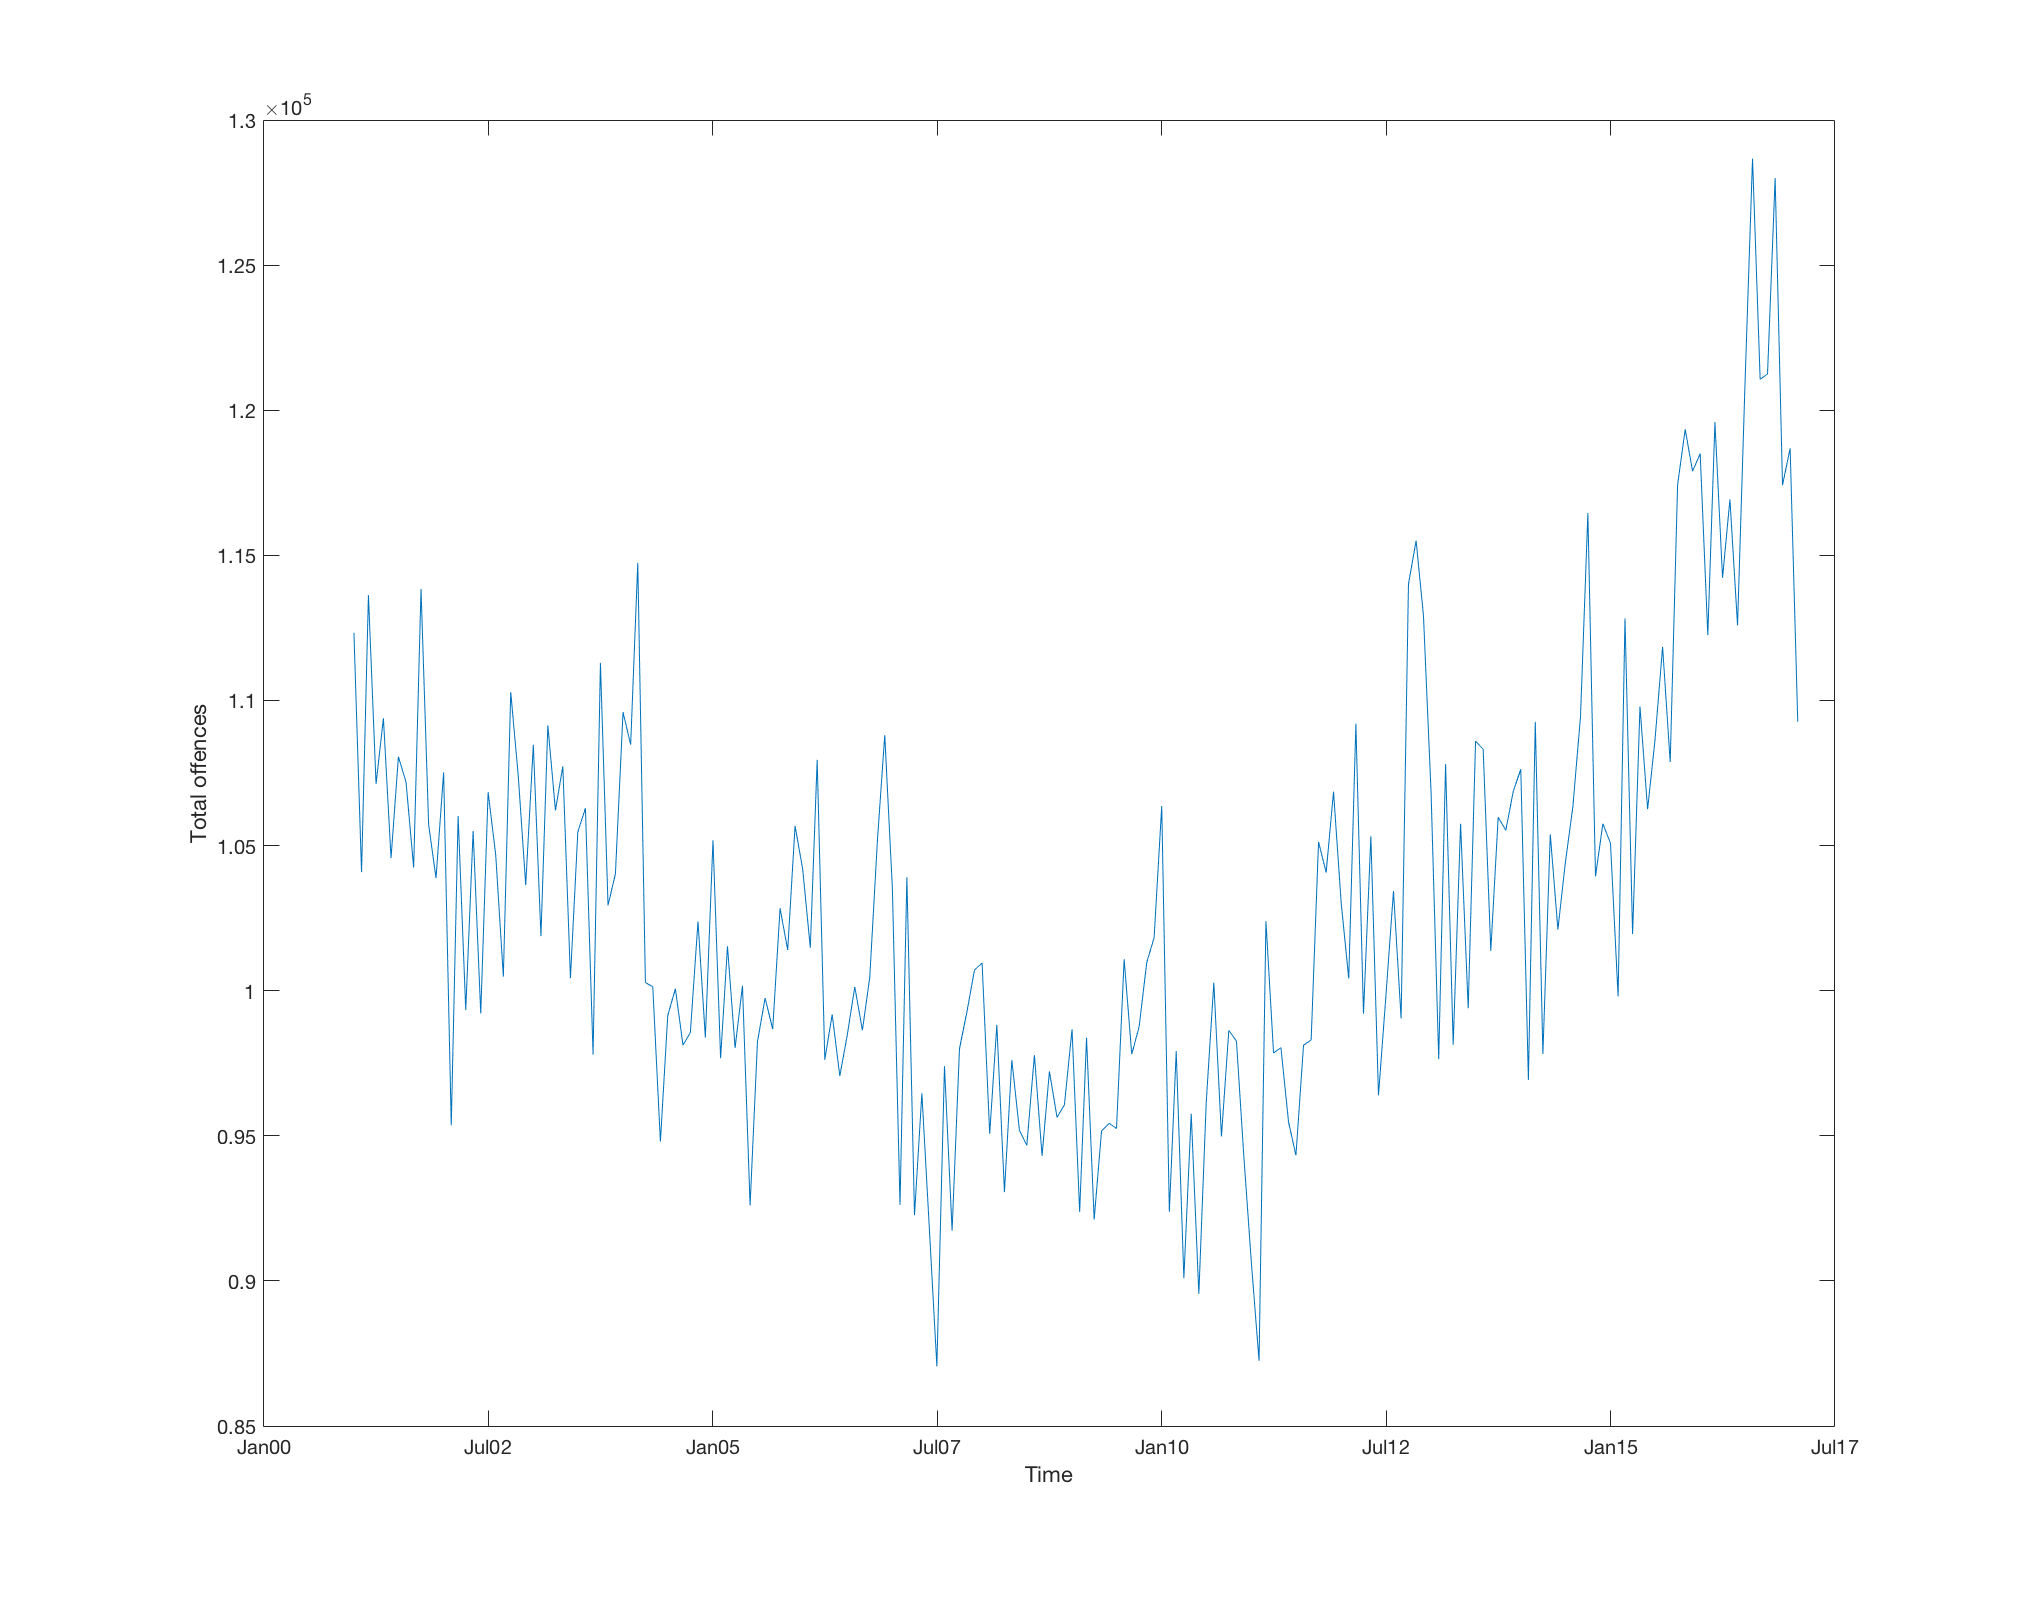
\includegraphics[width=\linewidth]{../images/crime_over_time}
\end{figure}

The chart shows that overall crime has been decreasing from 2001 through to 2010, 
but starting 2011 crime rates started increasing with the peak in 2016.

Additionally the chart shows that there is a lot of fluctuation from month to month.
To gain more insight into the crime trends, confidence intervals can be introduced to show the fluctuation in the data.

\begin{figure}[H]
    \caption{Total offences over time with 95\% confidence intervals}
    \centering
    \label{fig:crime_confidence}
    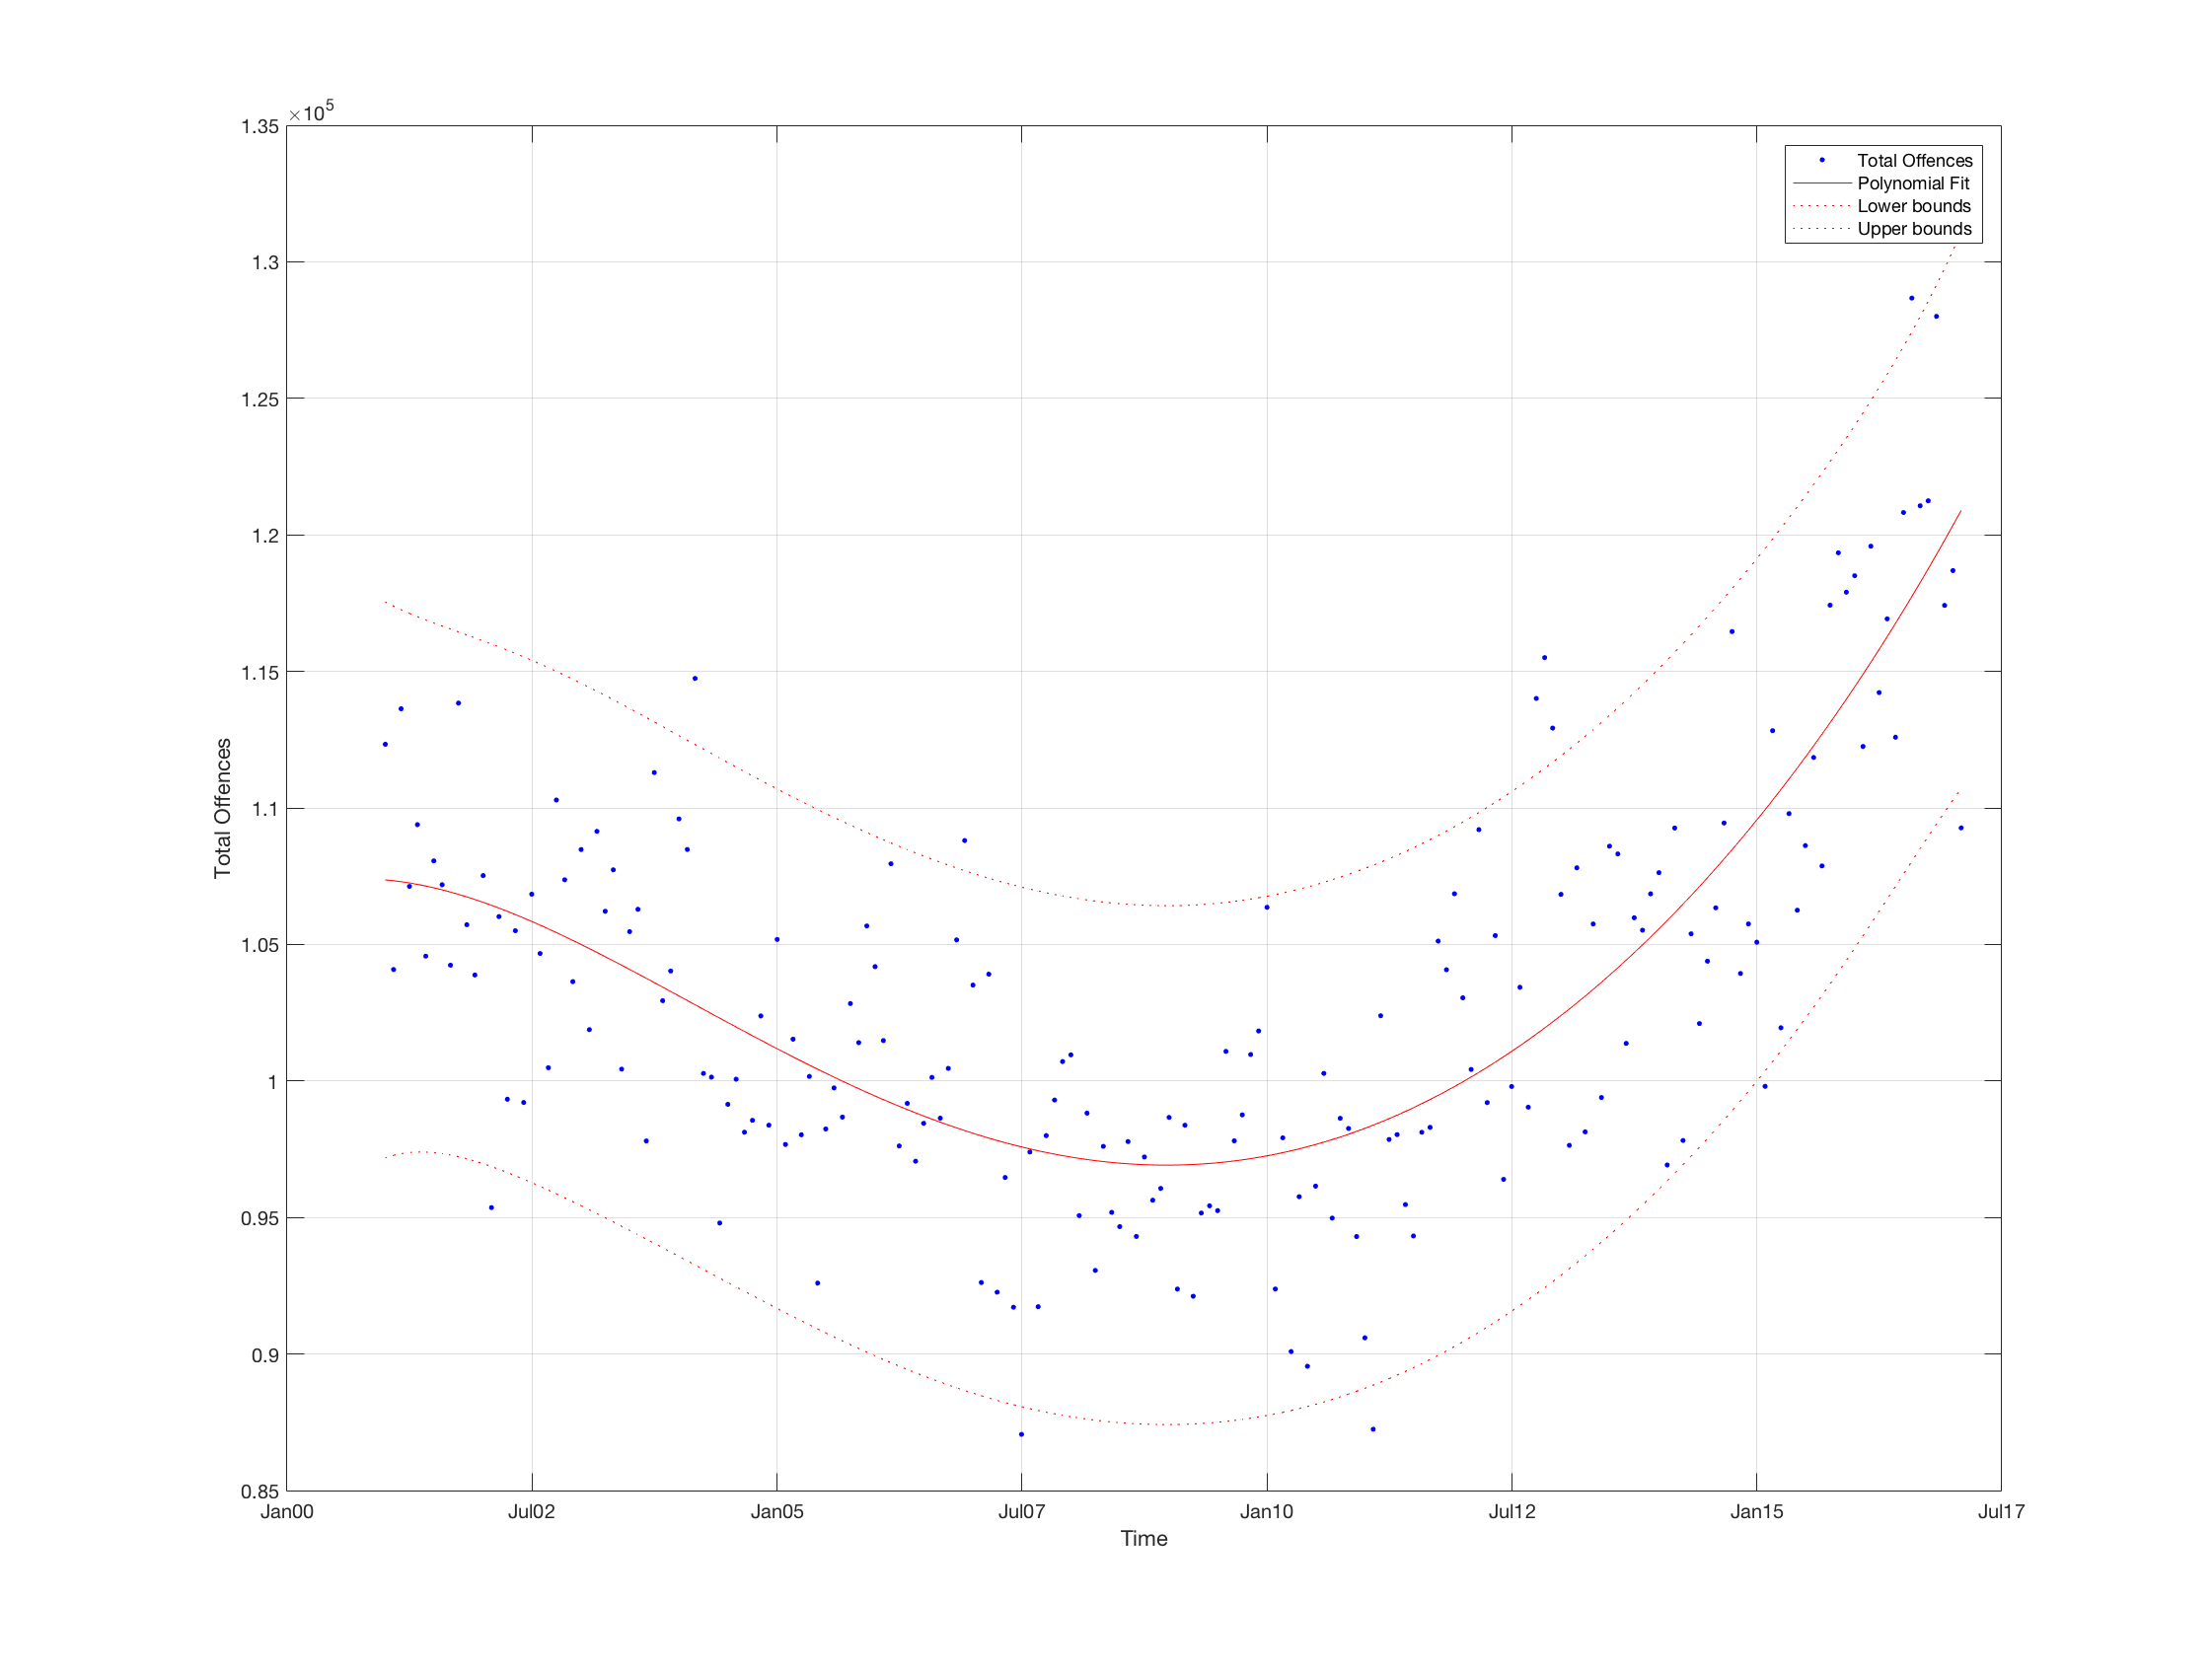
\includegraphics[width=\linewidth]{../images/crime_over_time_confidence}
\end{figure}

Figure~\ref{fig:crime_confidence} displays the 95\% confidence intervals when the data is plotted to a 5th 
degree polynomial.
The points above and below the confidence intervals are outliers, which could suggest that events occurred
during that time to cause the crime rates to increase or decrease.


Sorting the crimes by the average number of offences determined that the most common crimes are:

\begin{enumerate}
    \item Offences against property
    \item Other offences
    \item Other theft excluding unlawful entry
    \item Drug offences
    \item Unlawful entry
\end{enumerate}

These offences can be plotted against the months to see how they change over time.

\begin{figure}[H]
    \caption{Top offences over time}
    \centering
    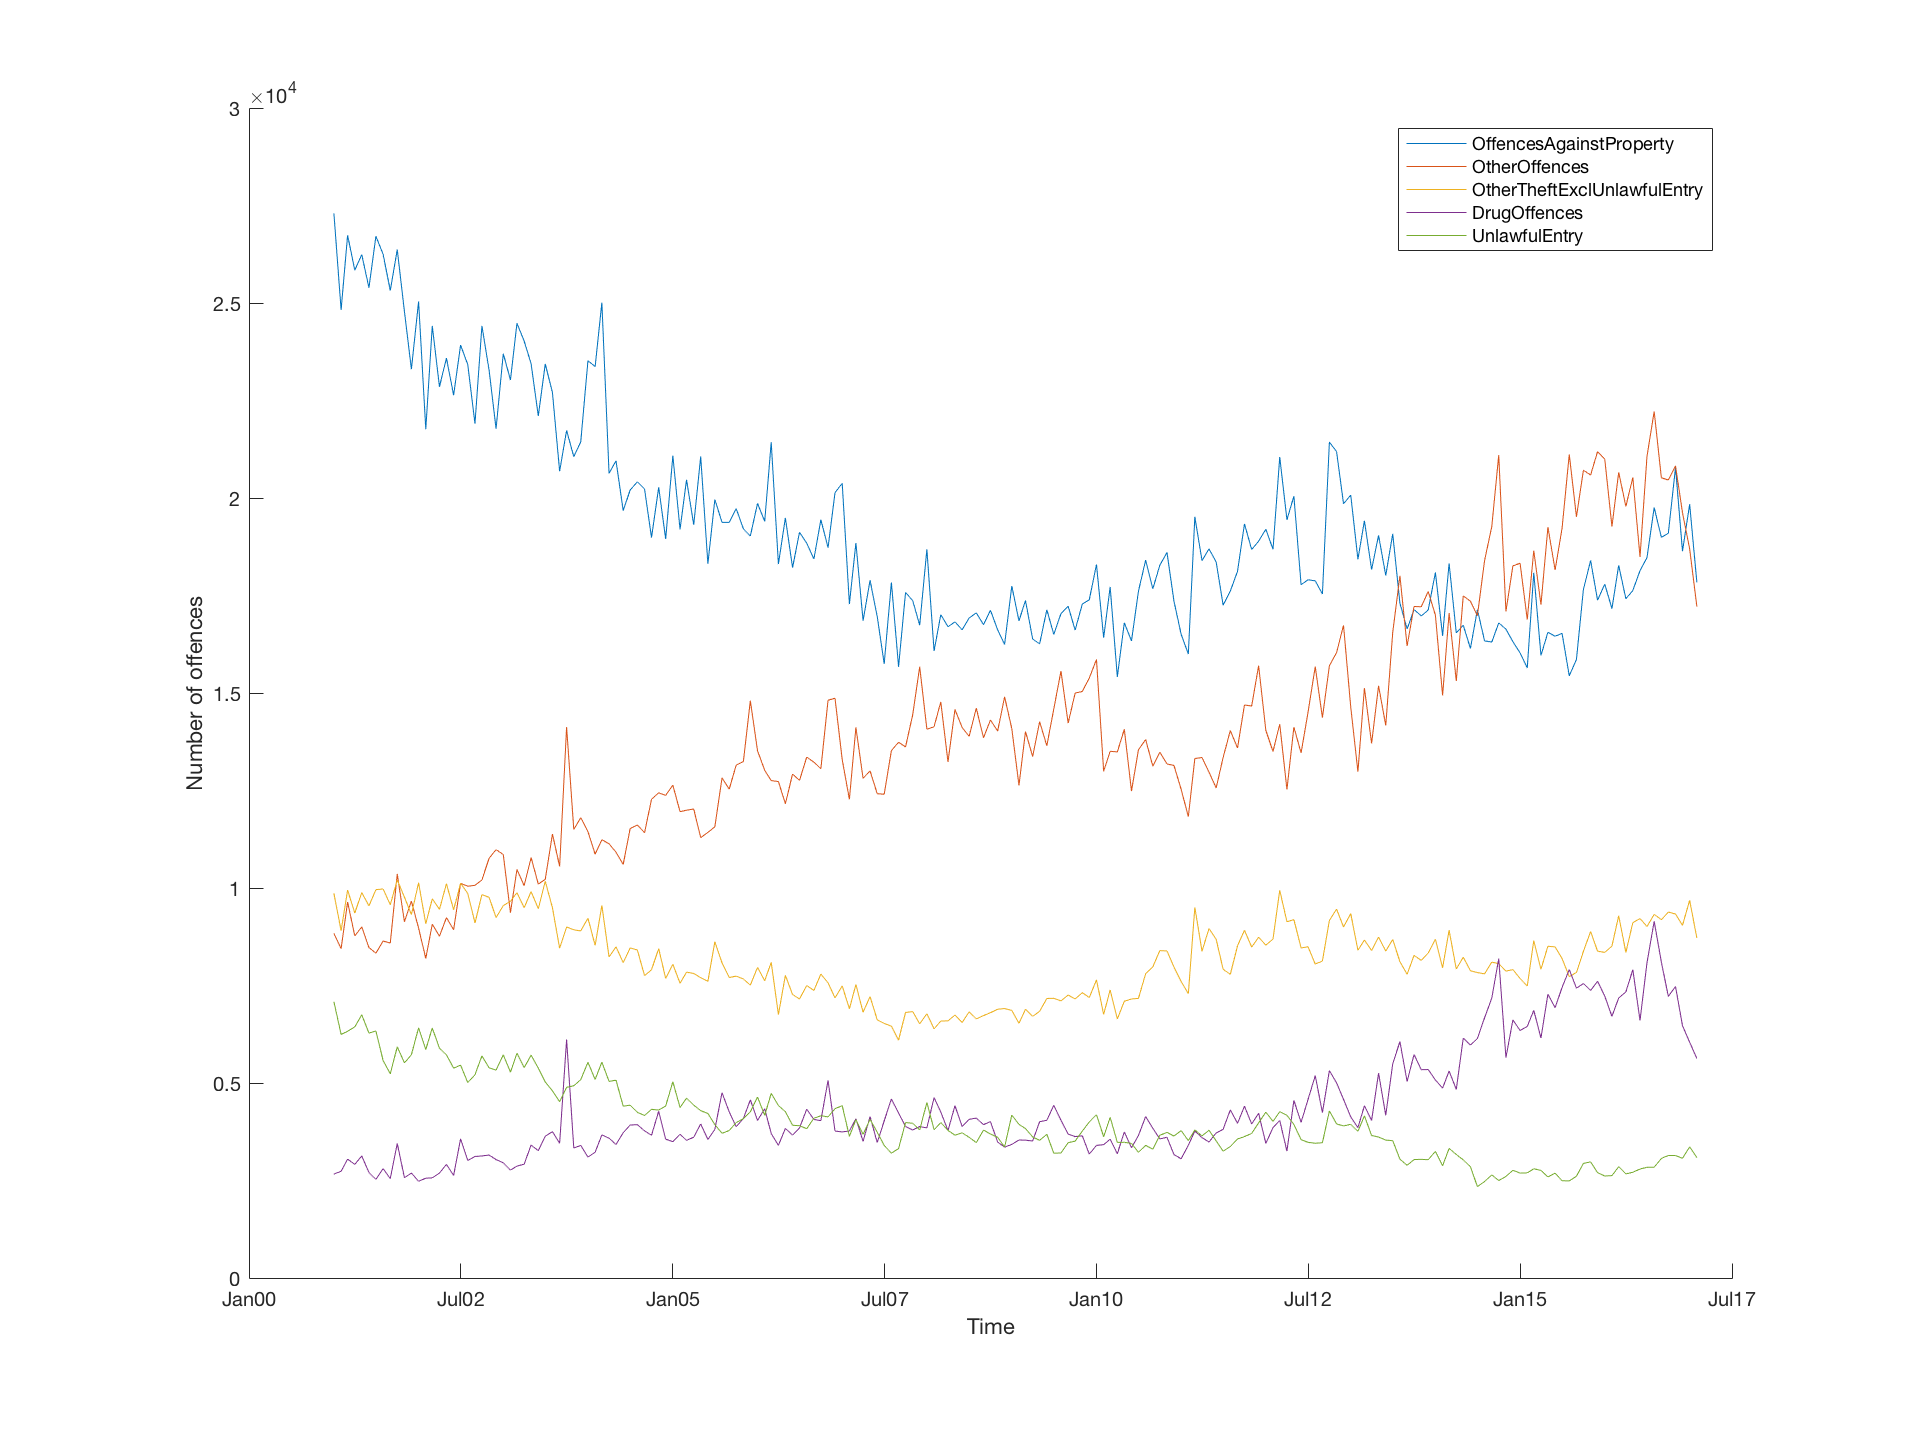
\includegraphics[width=\linewidth]{../images/top_offences_over_time}
\end{figure}

Displaying the types of offences over time shows a few trends.
Offences against properties has been on the decline, whereas other
types of offences has been increasing. Here `other' means the
offences that do not fit any existing categories according to the Queensland Police.
Additionally drug related offences has been increasing, but started to fall again at the start of 2017.

There is a spike in crime related offences between 2003 and 2004, where drug offences, other offences
and offences against properties all spiked for a short period. This suggests that
there could have been an event in 2003 that caused these to increase.

\begin{figure}[H]
    \caption{Recurrence Plot}
    \centering
    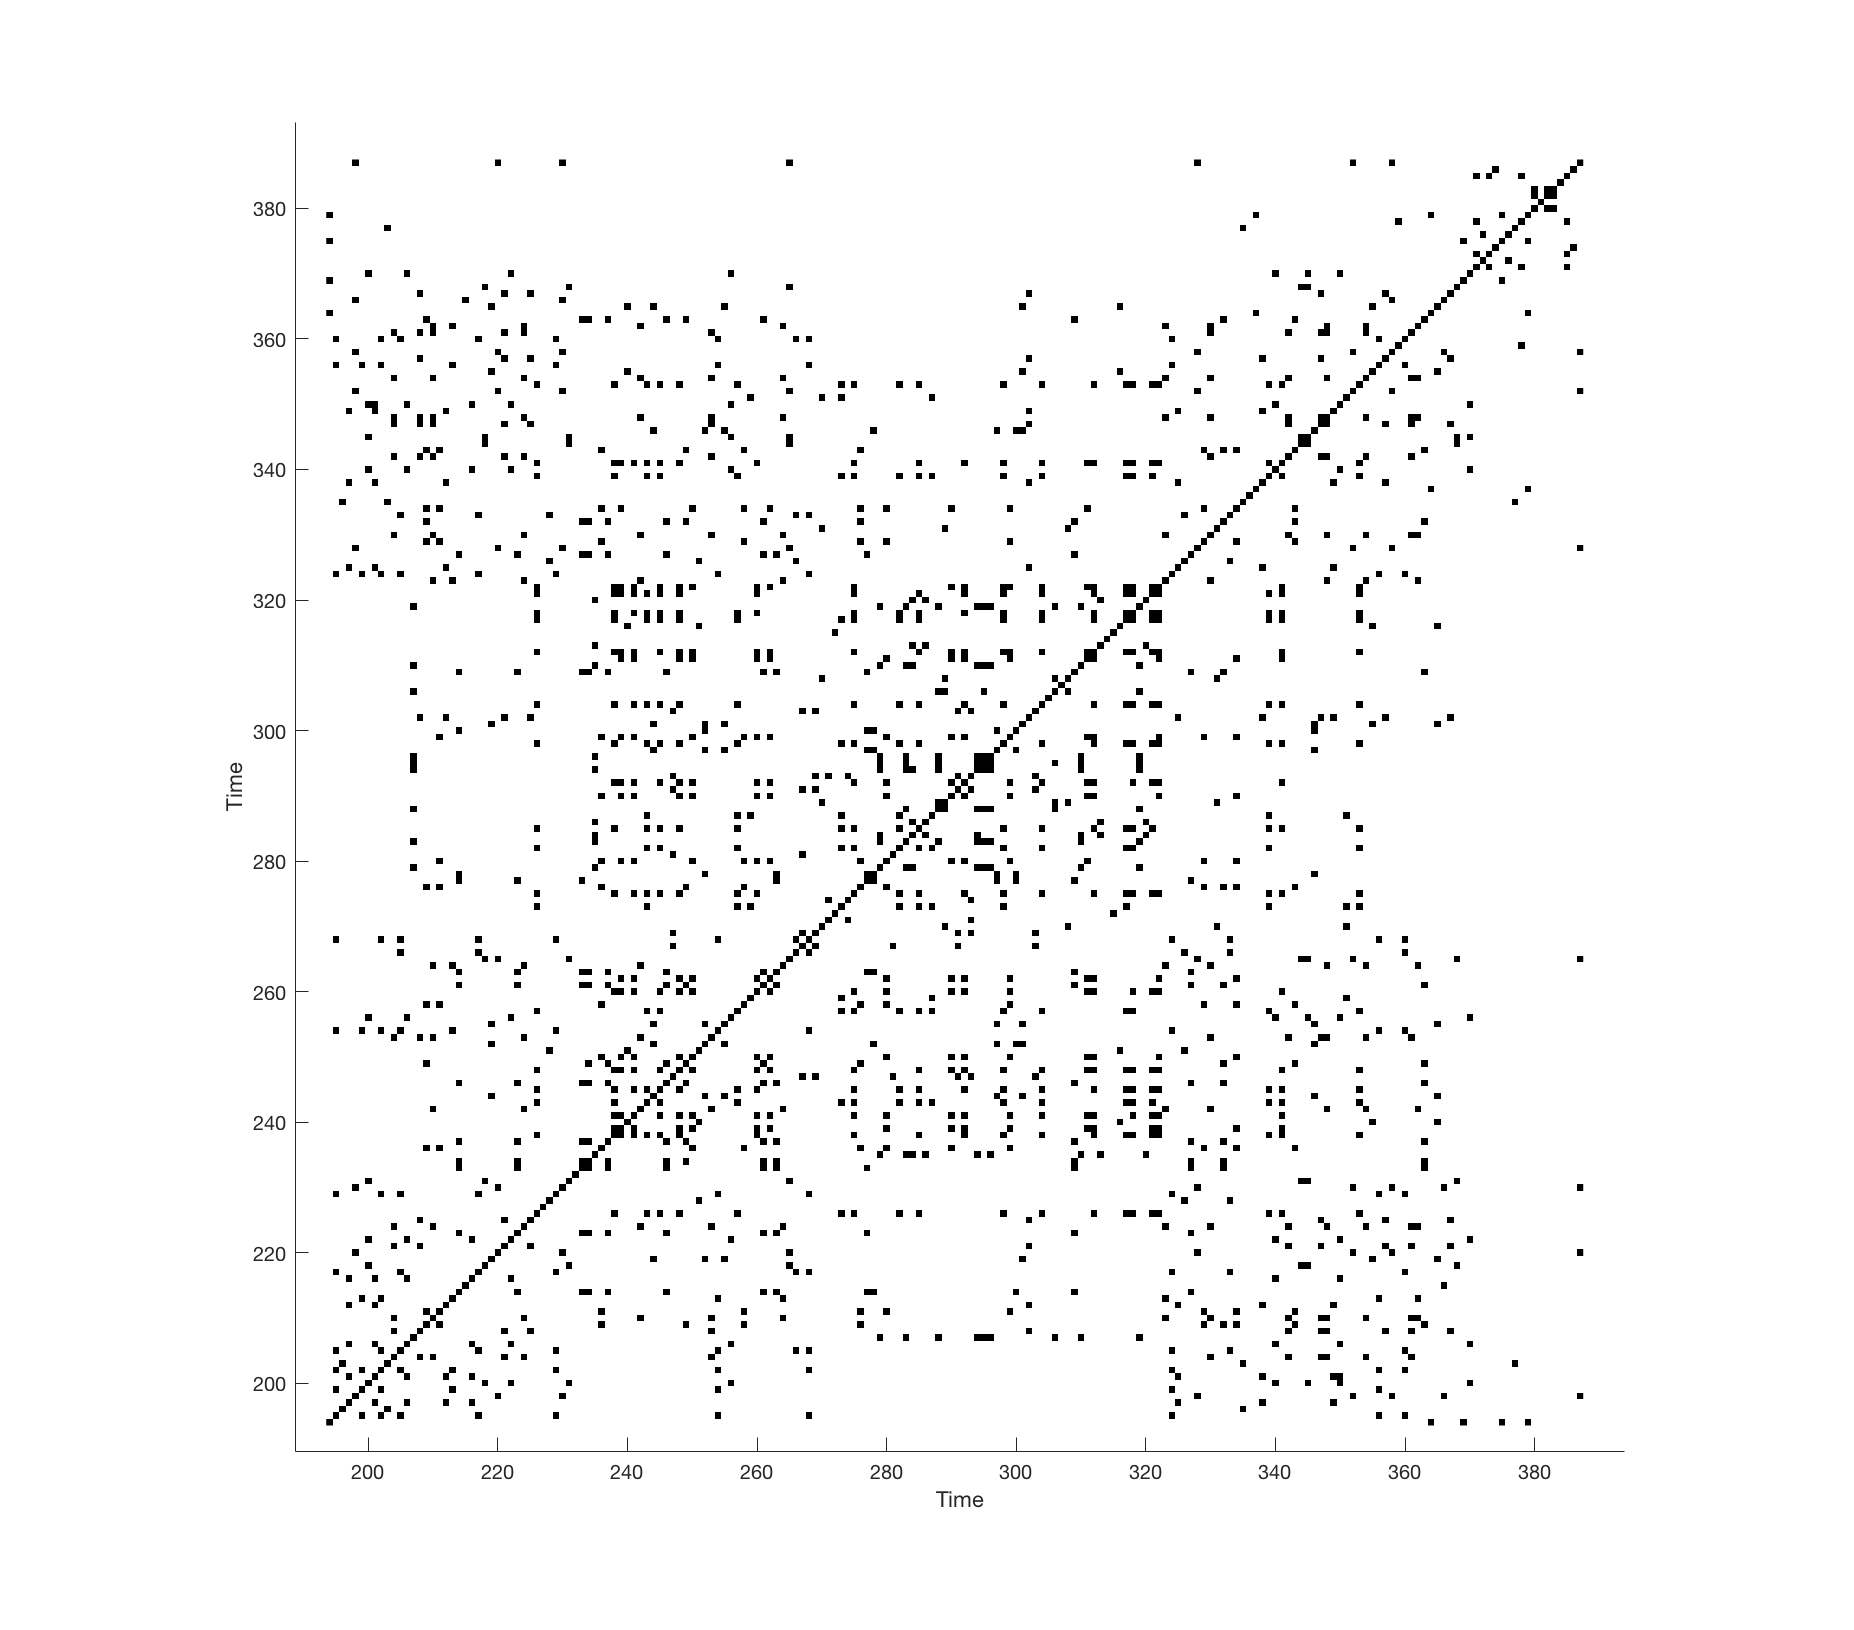
\includegraphics[width=\linewidth]{../images/recurrence_plot}
\end{figure}

The above graph is a recurrence plot of the crime data over time.
This shows how the data recurs over time.
More specifically it shows the regions of time when crime is at the lowest.

\subsection{Correlating crime data with police divisions}

The crime data can be correlated against police divisions on a map, which gives a
geospatial representation of the data.
For this analysis only the crimes occurring in February 2017 is used.

\begin{figure}[H]
    \caption{Police Division by Size}
    \centering
    \label{fig:police_divisions}
    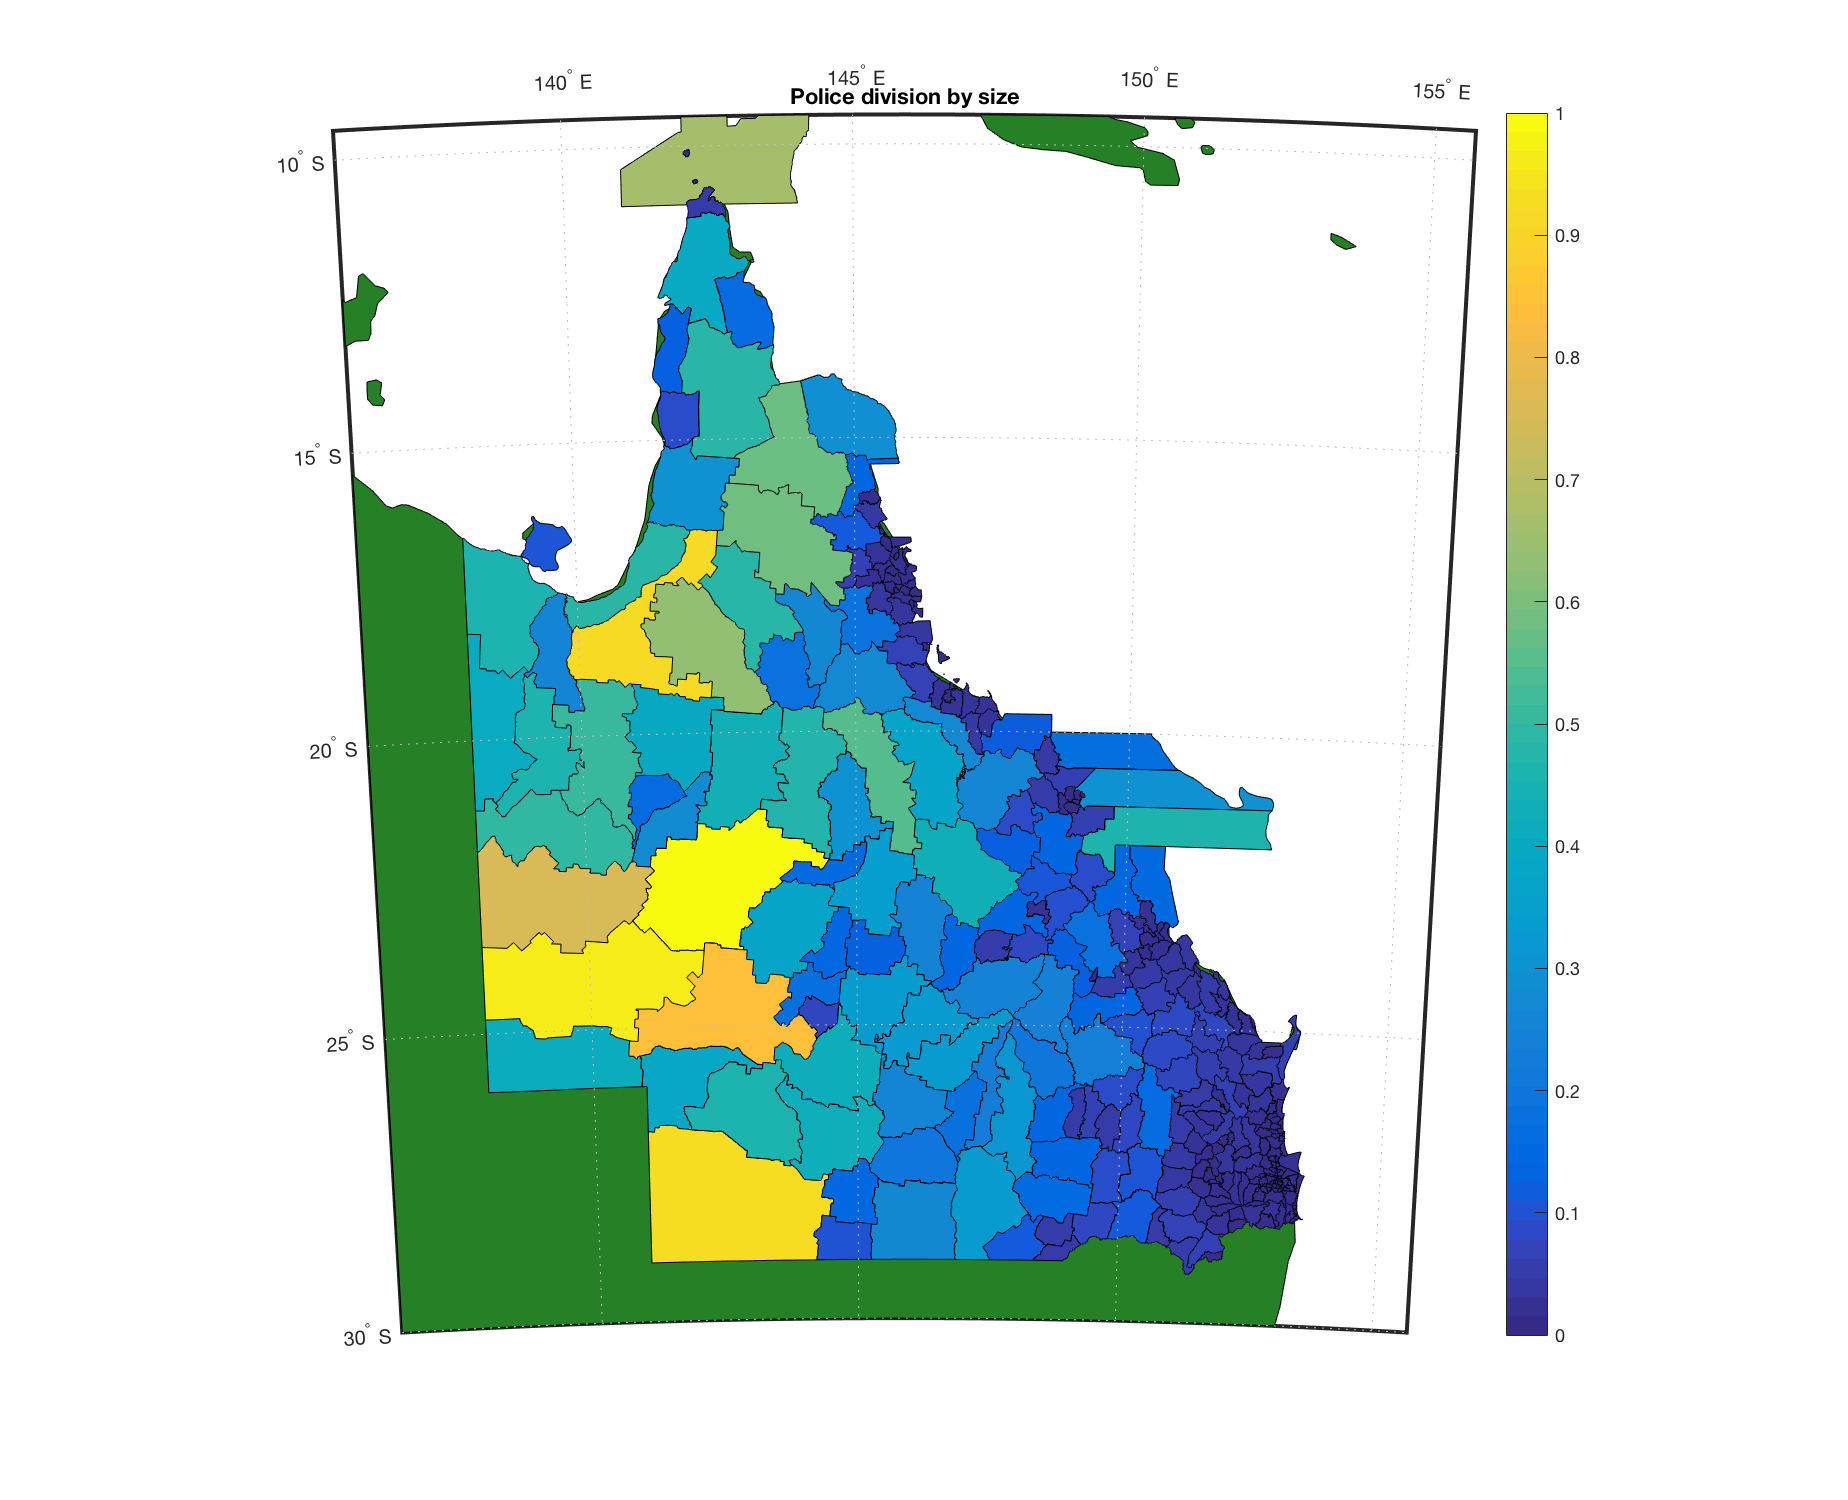
\includegraphics[width=\linewidth]{../images/police_division_by_size}
\end{figure}

The police divisions in Queensland can be plotted onto a map. The divisions with more land area are displayed in a lighter colour. The solid green is the base map, thus an area that the Queensland Police force does not patrol.

Larger police divisions indicate more rural areas with smaller populations, whereas smaller police divisions are within cities with a larger population density.
This makes sense as the crime rate increases as the population of a given area increases\cite{nolan_establishing_2004}.
So logically the Queensland Police will have more divisions where the crime rate is higher.

\begin{figure}[H]
    \caption{Police Division by Size (Brisbane Area)}
    \centering
    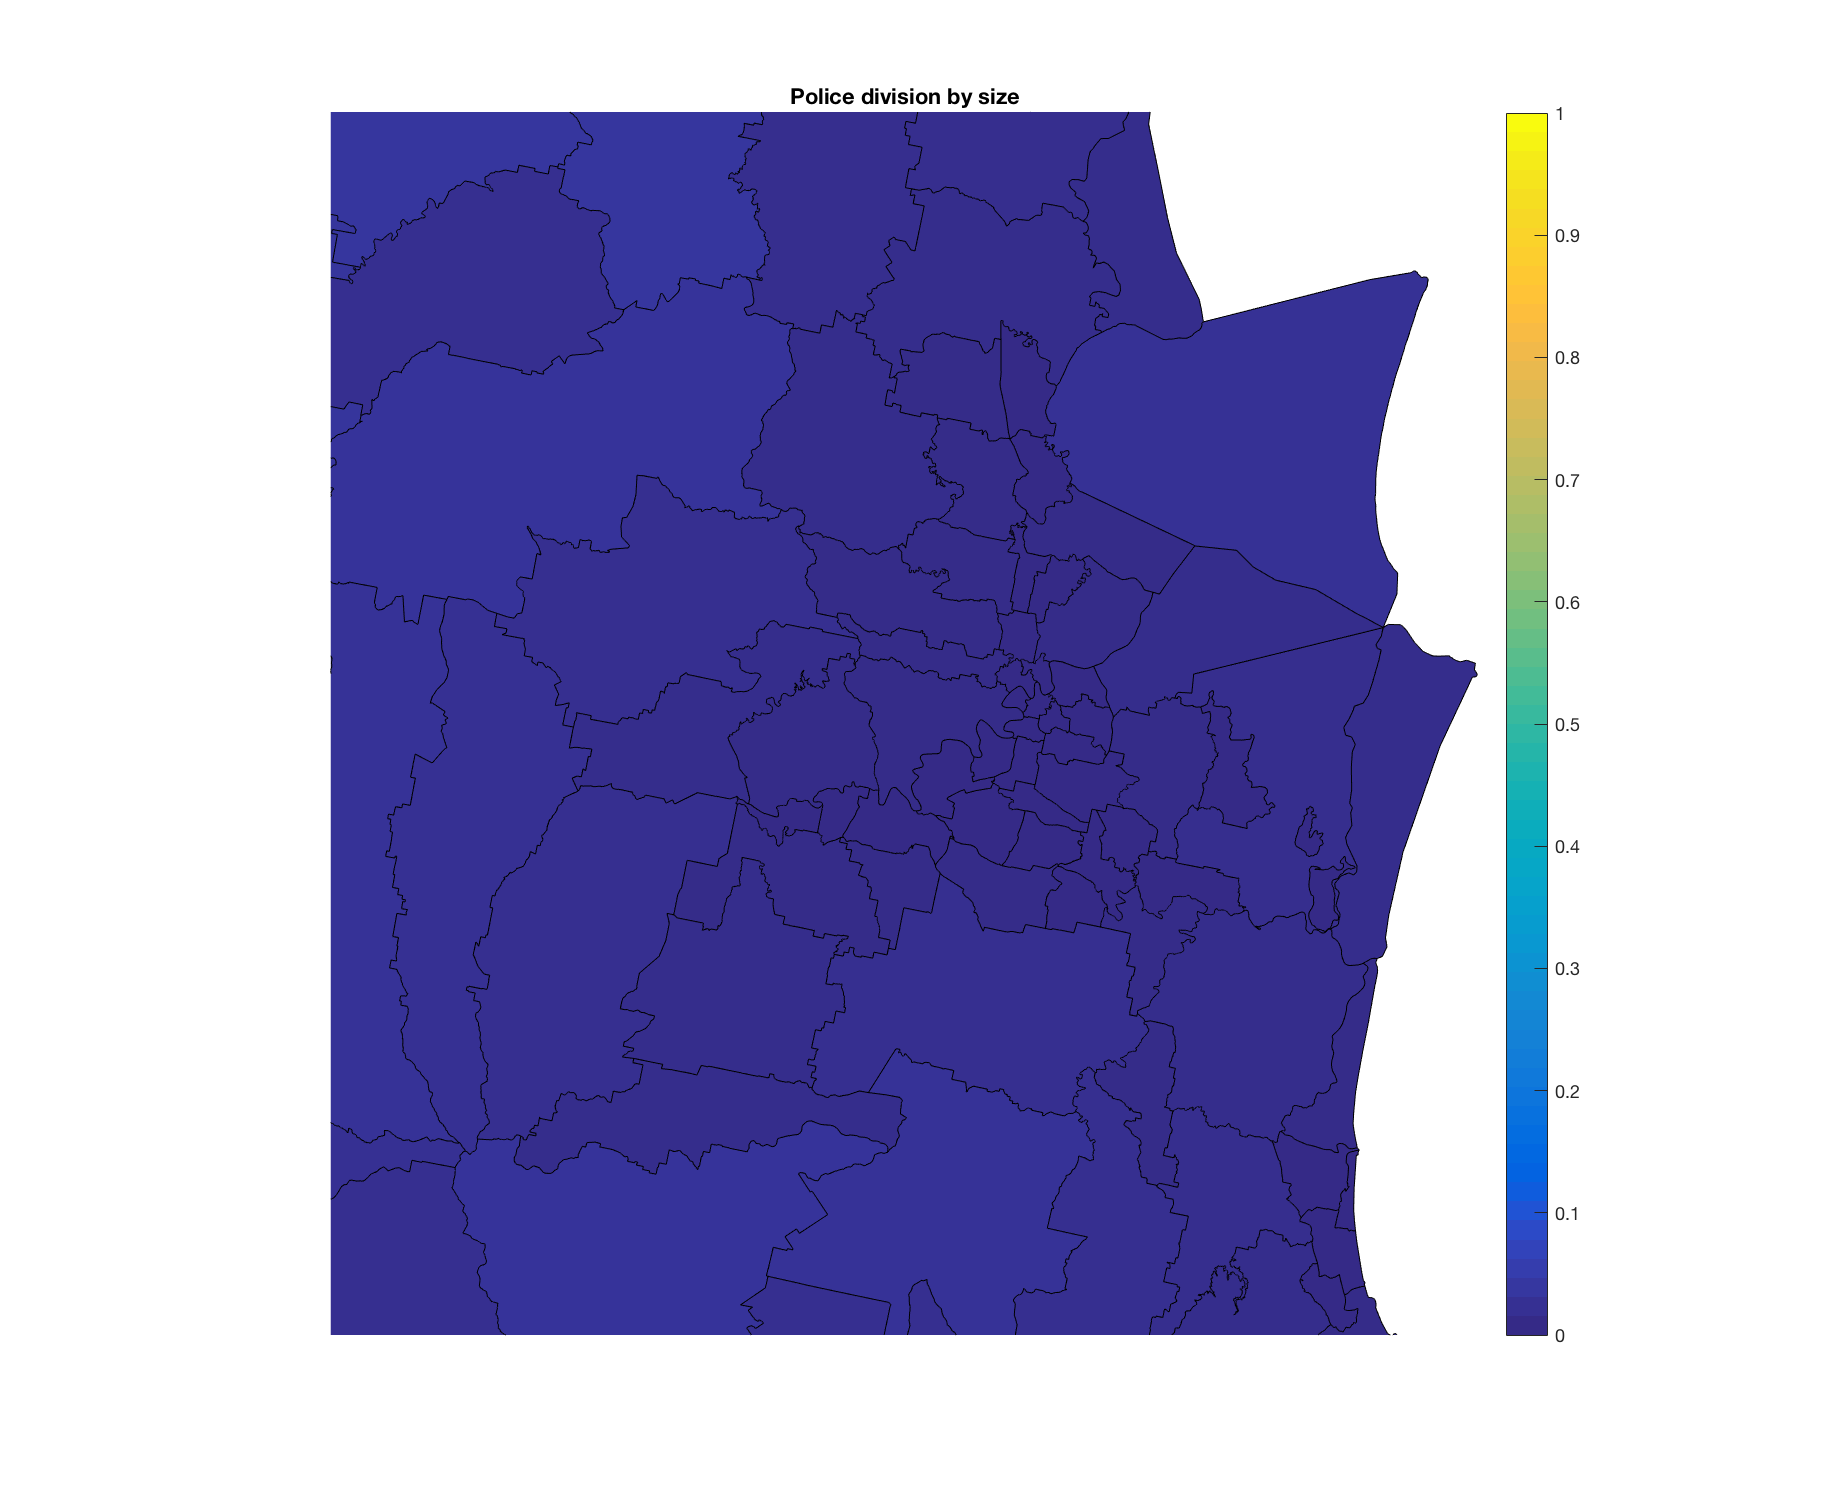
\includegraphics[width=\linewidth]{../images/police_division_by_size_brisbane}
\end{figure}

The police divisions around the Brisbane area are much smaller than anywhere else in Queensland, with the smallest ones being around Brisbane City and Fortitude Valley.

\begin{figure}[H]
    \caption{Police Division by Crime Density}
    \centering
    \label{fig:crime_density}
    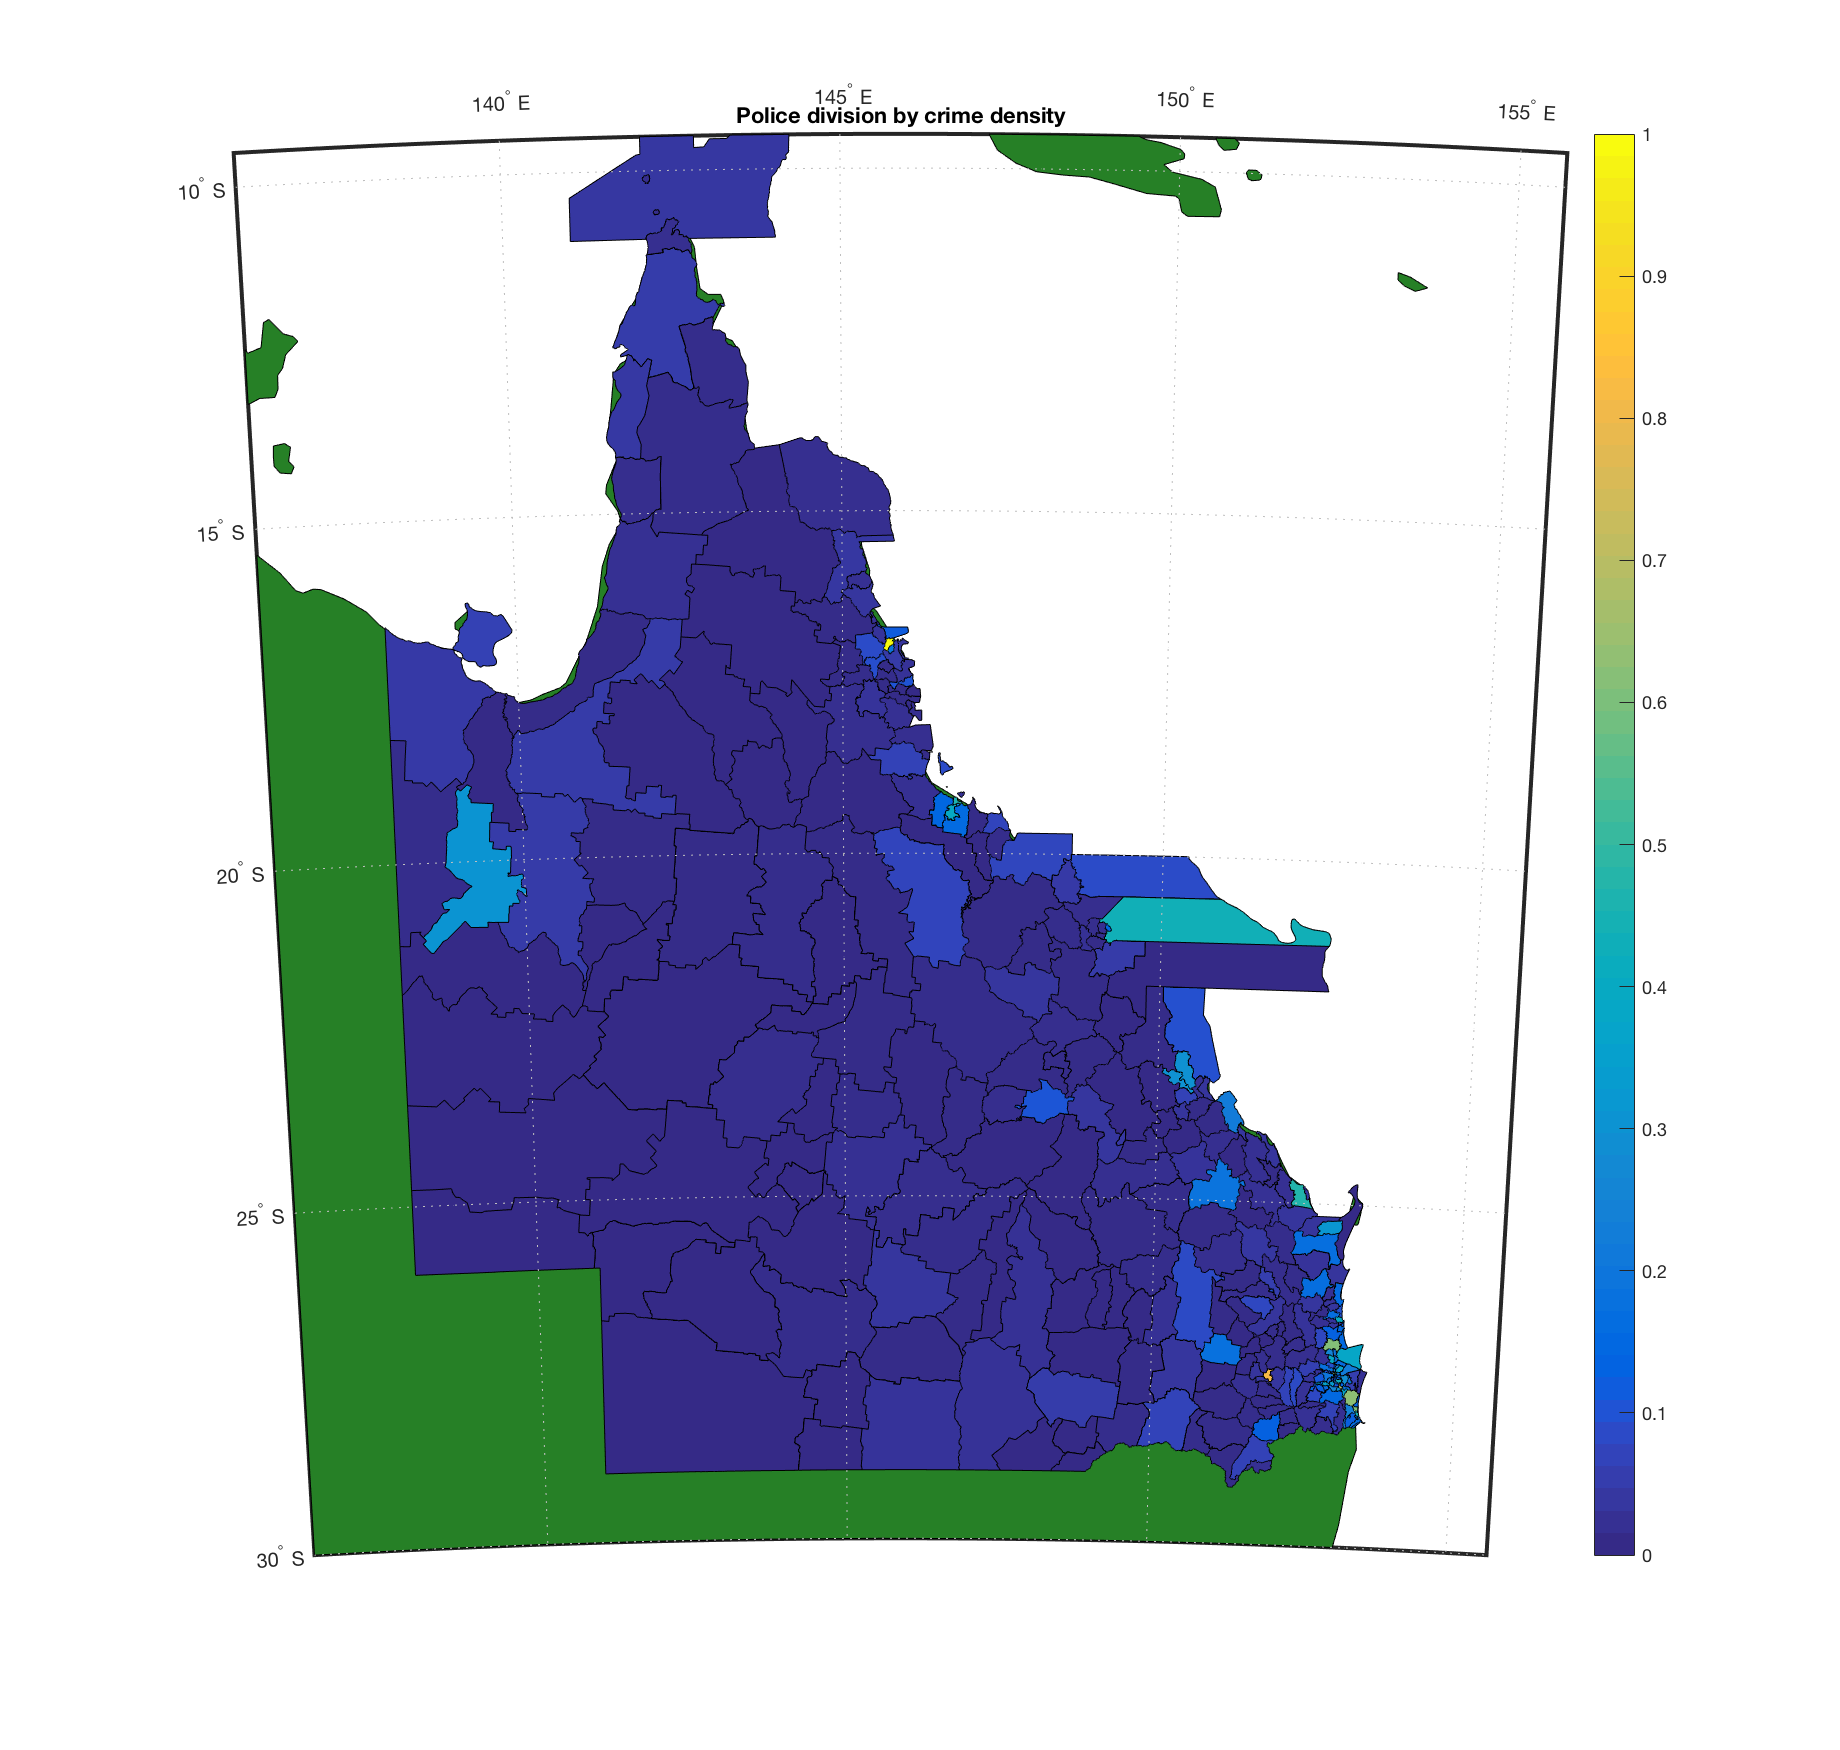
\includegraphics[width=\linewidth]{../images/police_division_by_crime_density}
\end{figure}

Figure~\ref{fig:crime_density} shows the density of crime in police divisions for February 2017, the lighter the colour, the more crime happens in that division.
Immediately it can be seen that there are a few brightly coloured points that stand out.

Furthermore by comparing figure~\ref{fig:police_divisions} and figure~\ref{fig:crime_density}, it can be seen that most of the police divisions with the largest land areas also has the lowest reported offences.
Thus suggesting that the more populated areas has more crime.
There are two large rural police divisions that do have higher crime rates.
One is Mount Isa, in the west, and the other is Mackay, in the east.
This could be an indication that those two rural divisions could be understaffed.

The ten police divisions with the most crime during the month of February 2017 was found to be:

\begin{table}[H]
    \caption{Divisions with most crime in February 2017}
    \centering
    \begin{tabular}{|c|c|}
        \hline
        Police District & Offences \\
        \hline
        Cairns & 4131 \\
        Toowoomba & 3383 \\
        Logan Central & 2829 \\
        Brisbane City & 2610 \\
        Coomera & 2598 \\
        Caboolture & 2538 \\
        Southport & 2495 \\
        Bundaburg & 1943 \\
        Townsville & 1922 \\
        Fortitude Valley & 1886 \\
        \hline
    \end{tabular}
\end{table}

\begin{figure}[H]
    \caption{Top crime in February 2017}
    \centering
    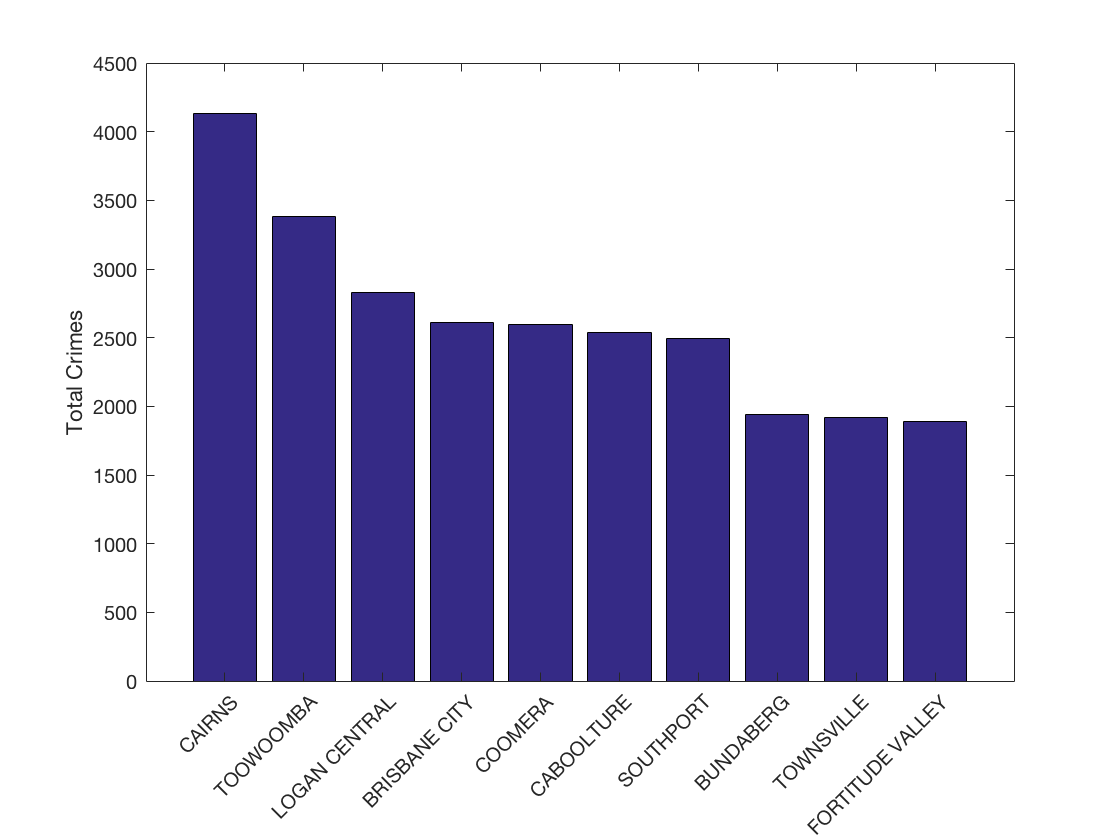
\includegraphics[width=\linewidth]{../images/top_crime_2017}
\end{figure}

This can be compared to the divisions with the most crime in February 2001. By comparing with the same month of the year, it should avoid any error cause by fluctuations caused by crime happening in certain months more than others.

\begin{table}[H]
    \caption{Divisions with most crime in February 2001}
    \centering
    \begin{tabular}{|c|c|}
        \hline
        Police District & Offences \\
        \hline
        Brisbane City & 5636 \\
        Cairns & 3833 \\
        Toowoomba & 3127 \\
        Surfers Paradise & 2613 \\
        Maroochydore & 2466 \\
        Fortitude Valley & 2266 \\
        Southport & 2234 \\
        Logan Central & 1999 \\
        Broadbeach & 1973 \\
        Hendra & 1851 \\
        \hline
    \end{tabular}
\end{table}

\begin{figure}[H]
    \caption{Top crime in February 2001}
    \centering
    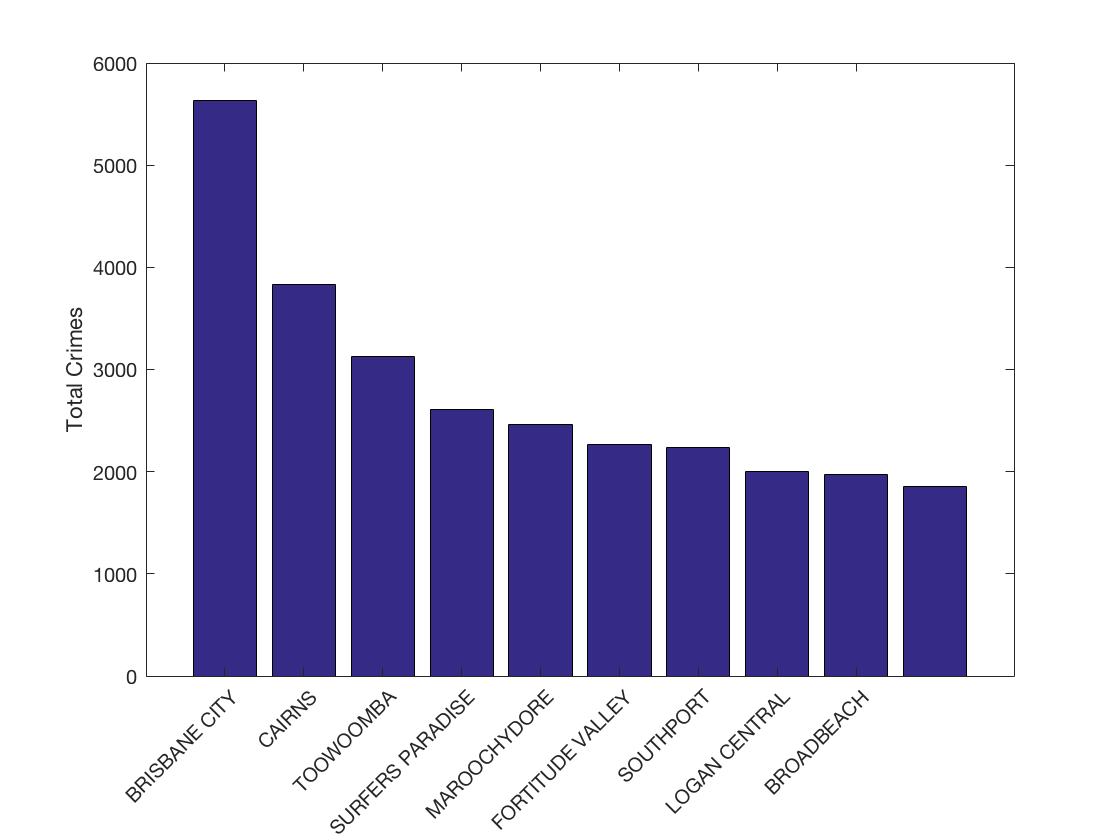
\includegraphics[width=\linewidth]{../images/top_crime_2001}
\end{figure}

The two tables show how crime rates change over time.
One of the largest changes is the crime in Brisbane City, which decreased significantly over 16 years.
Additionally Surfers Paradise and Maroochydore dropped off the list since 2001 and Coomera, Caboolture and Bundaburg had increases in crime over that period.

By comparing the data from multiple time periods, it can be seen how the crime rates of a division changes over time, as illustrated in the chart below.

\begin{figure}[H]
    \caption{Division Offences over Time}
    \centering
    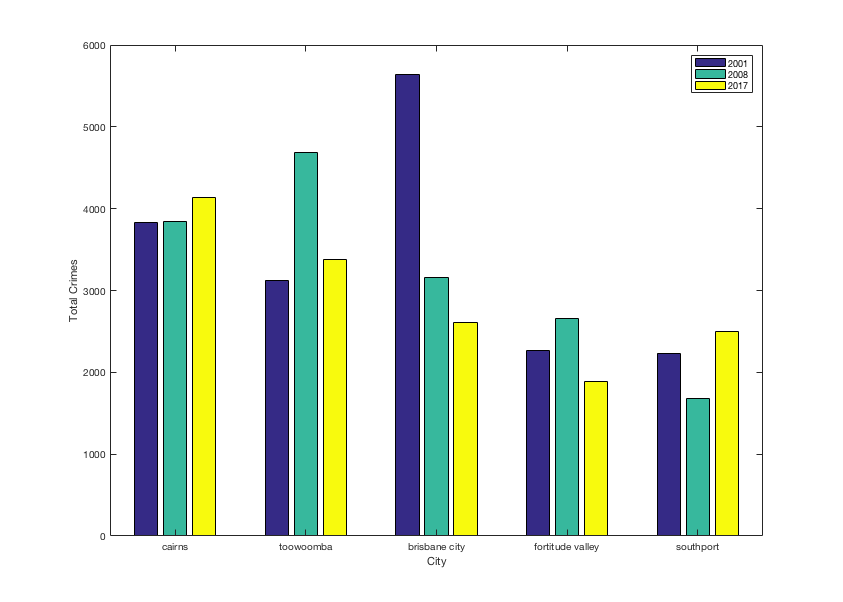
\includegraphics[width=\linewidth]{../images/top_crime_range}
\end{figure}

Above is a chart of how the offences in the top crime divisions change over time,
specifically comparing crime occurences during 2001, 2008 and 2017.
By choosing these equally spaced intervals we get a clearer picture of how the crime rate changes over time.
It can easily be seen that Brisbane City has the largest change in crime over time, with the crime rate being high in 2001 and steadily decreasing over time.
Cairns on the other hand has had a steadily high crime rate that increased over time.
Toowoomba had increased crime during 2008, but has since decreased.
Fortitude Valley and Southport has crime rates that oscillate over time.

\begin{figure}[H]
    \caption{Cairns crime density}
    \centering
    \label{fig:cairns_crime}
    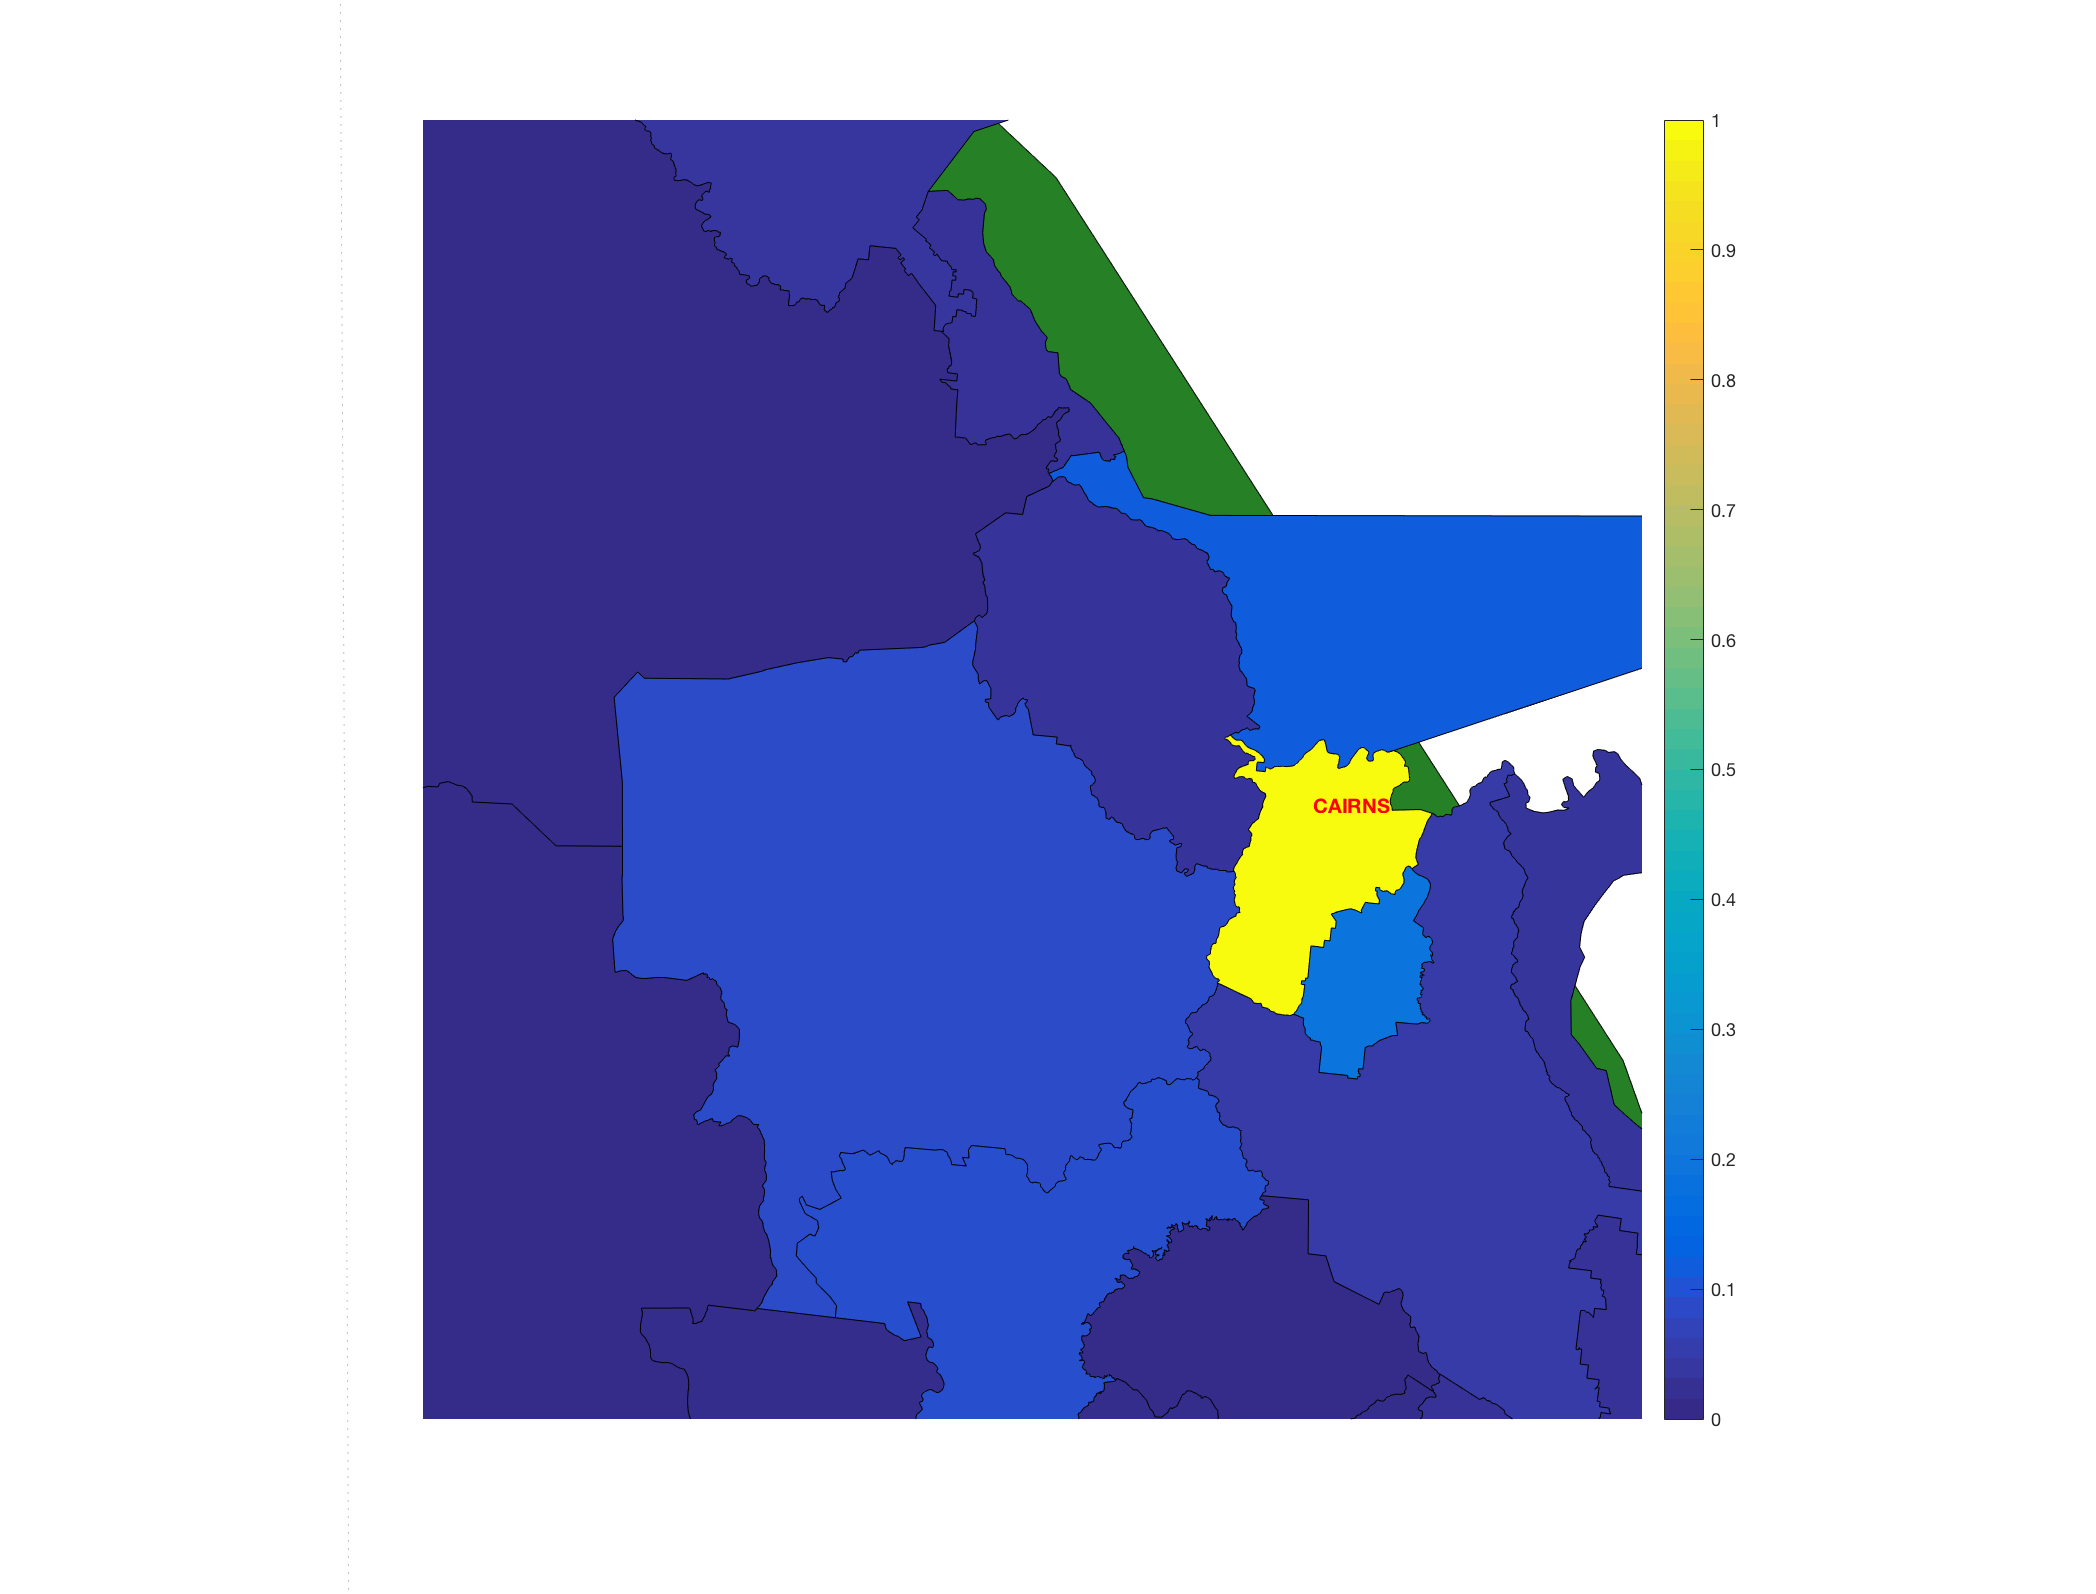
\includegraphics[width=\linewidth]{../images/cairns_crime}
\end{figure}

Figure~\ref{fig:cairns_crime} is interesting, as there is a large concentration of crime in one police division,
yet the surrounding area has significantly lower crime rates.
This differs from other areas, which has a much more gradual decrease in crime in surrounding areas, see figure~\ref{fig:brisbane_crime}.
Also note the solid green indicates there is no police division for that area, thus the map either has errors
or the area is a military base.

\begin{figure}[H]
    \caption{Brisbane crime density}
    \centering
    \label{fig:brisbane_crime}
    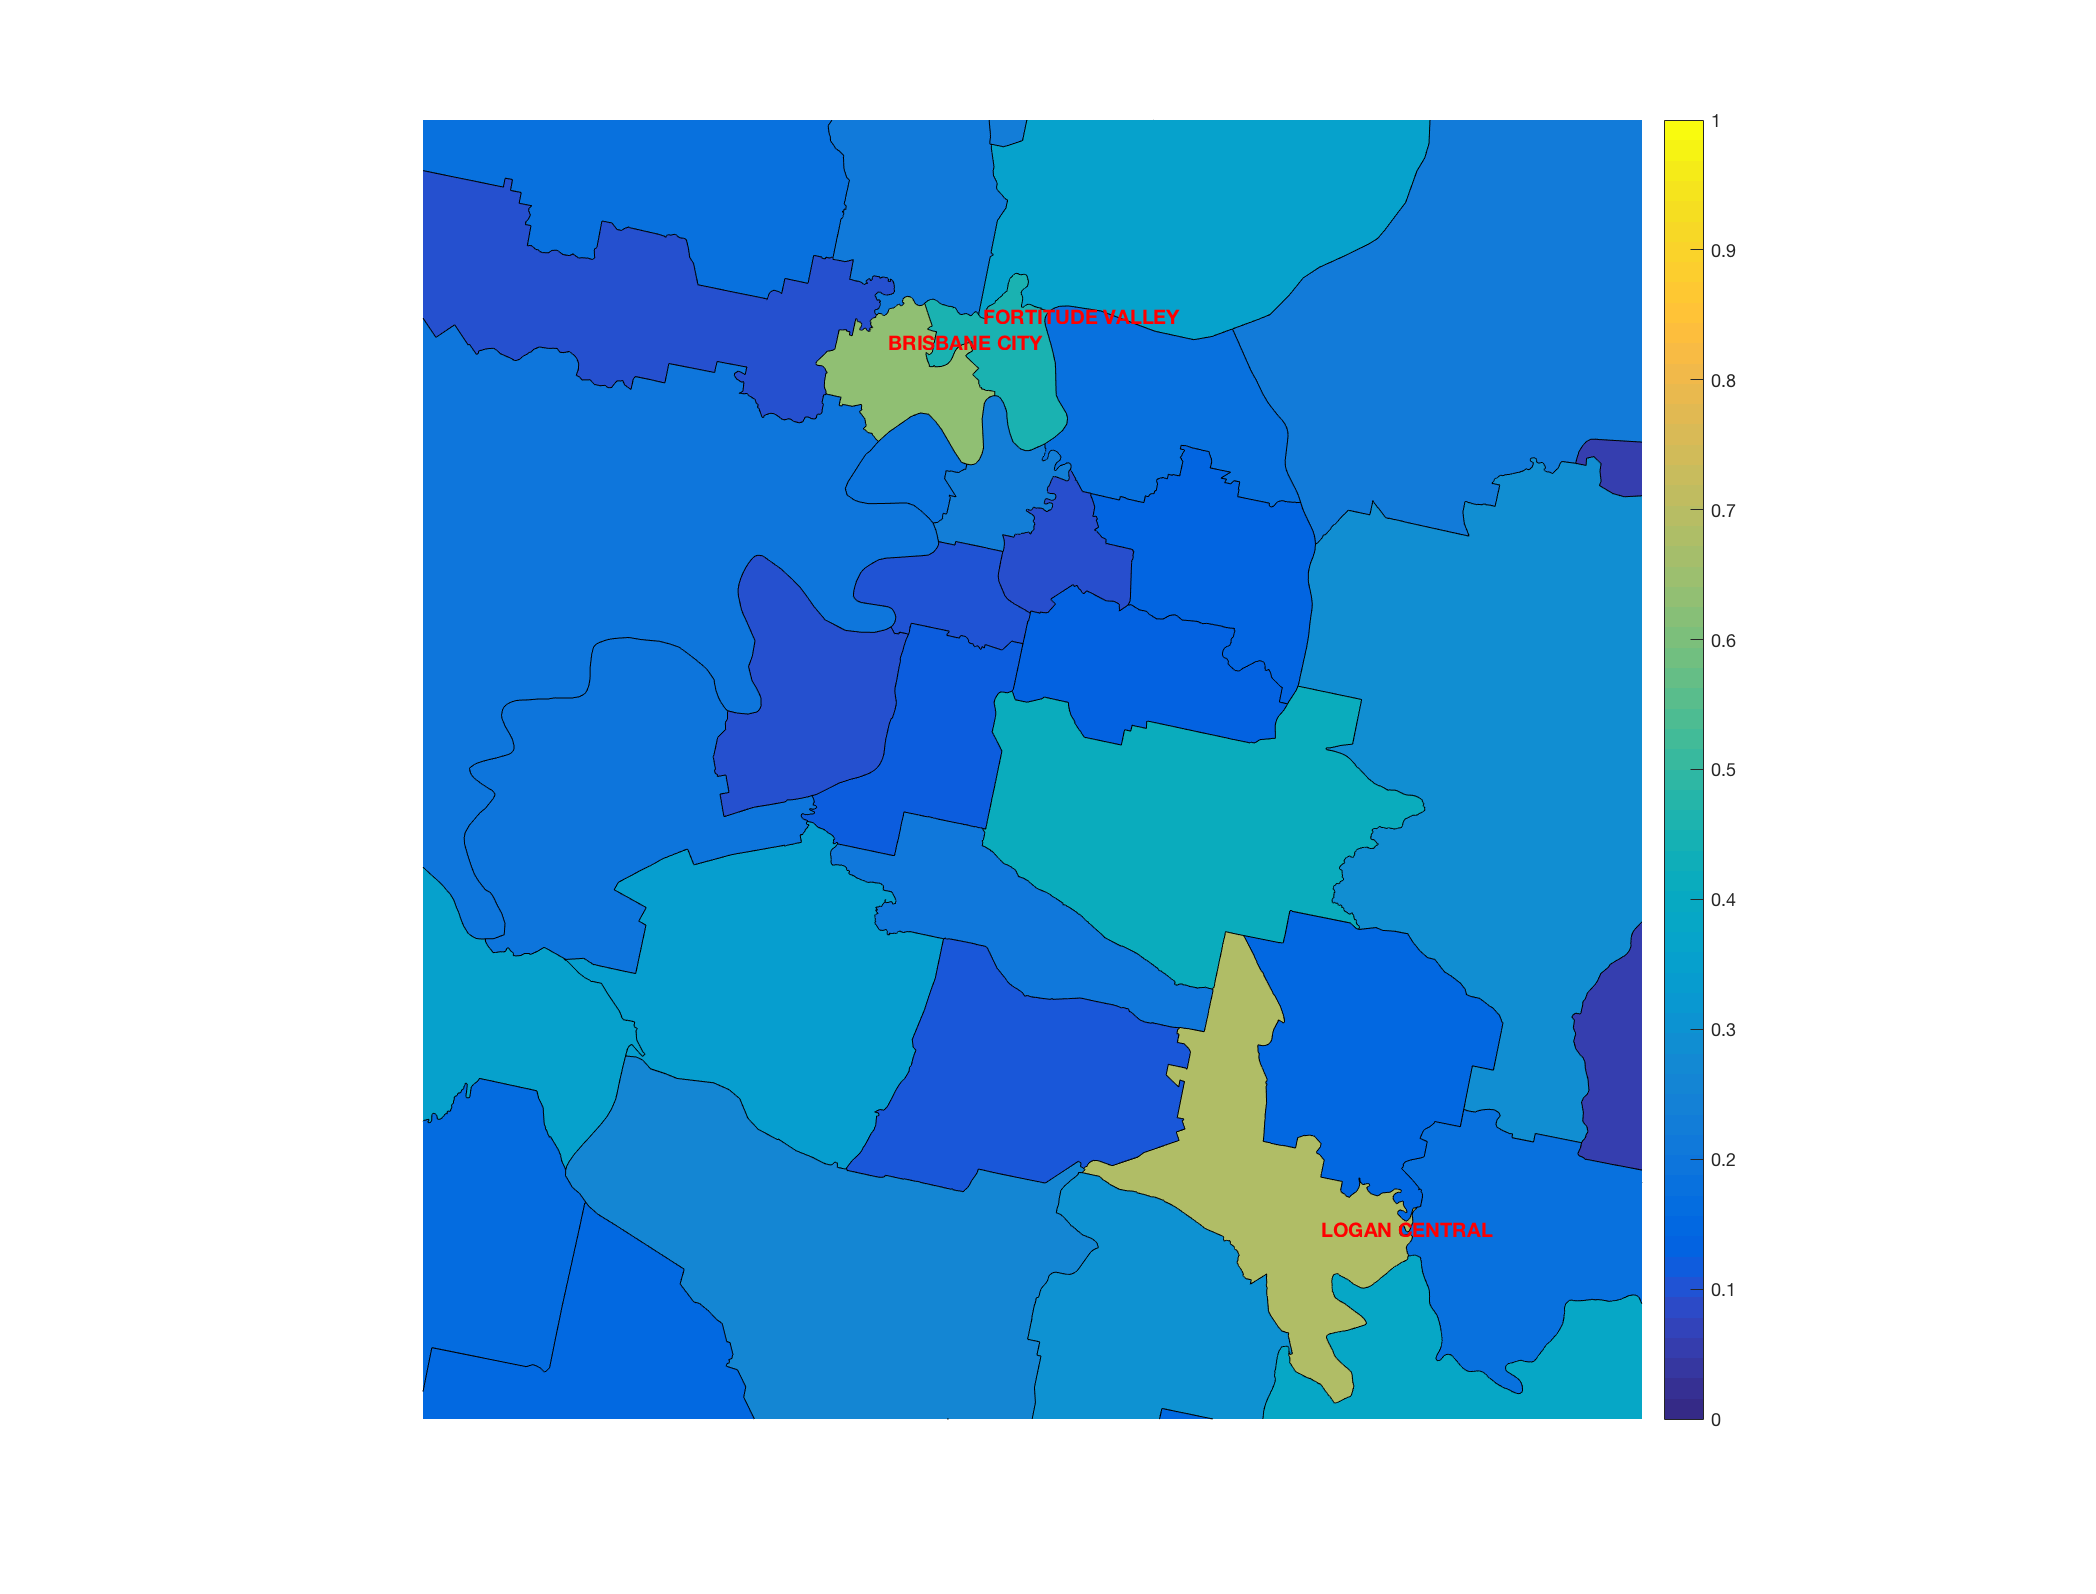
\includegraphics[width=\linewidth]{../images/brisbane_crime}
\end{figure}

The crime map for Brisbane shows that the areas with the most crime is Logan City, Brisbane City and Fortitude Valley.
Additionally neighboring areas also have increased crime rates, which is expected.

The map also shows that the divisions on the southside of the river generally have lower crime than northside suburbs.

\section{Limitations}

The accuracy of the crime data is limited to the police region, which doesn't allow fine grain analysis of the data.
Additionally since the rural police divisions are quite large, it is hard to determine where the crime occurred.
The New York government provides similar data, however they provide exact coordinates
of where crime happens, which allows much finer analysis of where crimes happen.

Additionally finer grain time periods would allow better analysis of data, as it would allow for more
accurate modelling of the data.

Furthermore the dataset only provided data for Queensland.
It would be more interesting to analyse and visualize crime for all of Australia.
This would yield more data and make it easier to determine what caused crime spikes.

\section{Conclusions}

Overall the analysis shows that crime in Queensland has been increasing since 2010.
Additionally the type of crime that increased in reported offences is `Other Crime', thus offences that does not fit any of Queensland Police's categories.
Drug related crime has also been increasing over time, but at a slower rate.

The crime analysis shows that Cairns has the most reported crime for any police division in Queensland, with 748 more offences than Toowoomba, the second most reported crime division.
Additionally unlike most of the other police regions the crime rates around the surrounding suburbs of Cairns is far lower than expected.
For example the high crime areas in Brisbane all have neighbouring suburbs with higher than normal levels of crime.

\section{References}

\bibliographystyle{abbrvurl}
\bibliography{bibliography}

\end{document}
